\documentclass[xcolor=table, 10pt, aspectratio=43]{beamer}

%\usepackage{arev}
\usepackage{amsmath,amssymb,amscd}
\usepackage{dsfont}
\usepackage{mathrsfs}
\usepackage{yfonts}
\usepackage{bm}
\usepackage{graphicx}
\usepackage{tabularx}
\usepackage{animate}
\usepackage{pifont}
%\usepackage{ifthen}

%\usepackage{xeCJK}
%\usepackage{fontspec}
%\newfontfamily\cjkfont{PingFang SC}
%\setCJKmainfont{PingFang SC}
\newcolumntype{x}{>{\centering\arraybackslash}X}
\renewcommand{\arraystretch}{1.5}

\usepackage{tikz}
	\usetikzlibrary{calc}
	\usetikzlibrary{arrows,shapes, positioning, matrix}
	\usetikzlibrary{decorations.markings}
	\tikzstyle arrowstyle=[scale=1]
	\tikzstyle directed=[postaction={decorate,decoration={markings,
 	   mark=at position .15 with {\arrow[arrowstyle]{stealth}}}}]
\tikzstyle string=[thick,postaction={decorate,decoration={markings,
    mark=at position .55 with {\arrow[arrowstyle]{stealth}}}}]
\tikzstyle dual_string=[dashed,postaction={decorate,decoration={markings,
    mark=at position .55 with {\arrow[arrowstyle]{stealth}}}}]

\tikzstyle dw=[thick,postaction={decorate,decoration={markings,
    mark=at position 1 with {\arrow[arrowstyle]{stealth}}}}]
\tikzstyle group=[mbg]

\usepackage{pgffor}
\newcommand{\mb}[1]{\mathbf{#1}}
\renewcommand{\cal}[1]{\mathcal{#1}}

\newcommand{\ag}[2]{#1_\mb{#2}}
\newcommand{\cohosub}[1]{\scalebox{0.72}{\textswab{#1}}}
\newcommand{\cohosubsub}[1]{\scalebox{0.6}{\textswab{#1}}}
\newcommand{\coho}[1]{\textswab{#1}}


\mode<presentation>
{
  %\usetheme{Warsaw}
  % or ...
  %\useoutertheme{rectangle}
  \setbeamertemplate{frametitle}[default][center]
  \defbeamertemplate{itemize item}{flat}{\begin{pgfpicture}{-1ex}{0ex}{1ex}{2ex}
      \pgfpathcircle{\pgfpoint{0pt}{.6ex}}{0.6ex}
      \pgfusepath{fill}
    \end{pgfpicture}%
  }
  \defbeamertemplate{itemize subitem}{flat}{\footnotesize\raise0.5pt\hbox{\textbullet}}
  \defbeamertemplate{itemize subsubitem}{flat}{\footnotesize\raise0.5pt\hbox{\textbullet}}

  %\useinnertheme{circles}
  \setbeamertemplate{items}[flat]
  \setbeamertemplate{sections/subsections in toc}[circle]
  \setbeamertemplate{blocks}[rounded]
  \setbeamertemplate{title page}[default][colsep=-4bp,rounded=true]
  \setbeamertemplate{part page}[default][colsep=-4bp,rounded=true]
  \setbeamercovered{transparent}
  %\usecolortheme{spruce}
  %\definecolor{THU}{RGB}{116,61,130}
  \definecolor{mbg}{RGB}{0,0,160}
  \setbeamercolor*{palette primary}{fg=white,bg=mbg}
  \setbeamercolor*{titlelike}{parent=palette primary}
  \setbeamercolor*{structure}{fg=mbg}
  \setbeamercolor{frametitle}{fg=white,bg=mbg}
  % or whatever (possibly just delete it)
  \setbeamercolor{block title}{bg=mbg,fg=white}
  \setbeamercolor{block body}{bg=mbg!15}


  \addtobeamertemplate{navigation symbols}{}{ \hspace{1em}%
    \usebeamerfont{footline}%
    \insertframenumber / \inserttotalframenumber }
}


%\usepackage[english]{babel}
% or whatever

%\usepackage[latin1]{inputenc}
% or whatever

%\usepackage{times}
%\usepackage[T1]{fontenc}
% Or whatever. Note that the encoding and the font should match. If T1
% does not look nice, try deleting the line with the fontenc.

\title[EQMC] % (optional, use only with long paper titles)
{DQMC simulation of U(1)-Dirac Quantum Spin Liquids and Orthogonal Metals}

\author[Y Qi] % (optional, use only with lots of authors)
{Yang~Qi}
% - Give the names in the same order as the appear in the paper.
% - Use the \inst{?} command only if the authors have different
%   affiliation.

\institute[Fudan] % (optional, but mostly needed)
{
Department of Physics, Fudan University.
}
% - Use the \inst command only if there are several affiliations.
% - Keep it simple, no one is interested in your street address.

%\date{2016 Annual Meeting of Fudan CFTPP} % (optional, should be abbreviation of conference name)
%{Fudan University, Oct 13 2015}
\date{IASTU, July 15th 2019.}
% - Either use conference name or its abbreviation.
% - Not really informative to the audience, more for people (including
%   yourself) who are reading the slides online

\subject{Theoretical Physics}
% This is only inserted into the PDF information catalog. Can be left
% out.



% If you have a file called "university-logo-filename.xxx", where xxx
% is a graphic format that can be processed by latex or pdflatex,
% resp., then you can add a logo as follows:

\pgfdeclareimage[height=1cm]{university-logo}{../resources/fudan}
\logo{\pgfuseimage{university-logo}}



% Delete this, if you do not want the table of contents to pop up at
% the beginning of each subsection:
\AtBeginSection[]
{
  \begin{frame}<beamer>{Outline}
			\tableofcontents[currentsection,currentsubsection]
  \end{frame}
}
\AtBeginSubsection[]
{
  \begin{frame}<beamer>{Outline}
    \tableofcontents[currentsection,currentsubsection]
  \end{frame}
}


\begin{document}

\begin{frame}
  \titlepage
\end{frame}

\begin{frame}{Collaborators}
\begin{itemize}
\item Xiao Yan Xu, Hong Kong University of Science and Technology.
\item Zi Yang Meng, Institute of Physics, Beijing.
\item Long Zhang, Kavli Institute for Theoretical Sciences, UCAS, Beijing.
\item Fakher F. Assaad, Universit\"at W\"urzburg.
\item Cenke Xu, University of California, Santa Barbara.
\begin{center}
  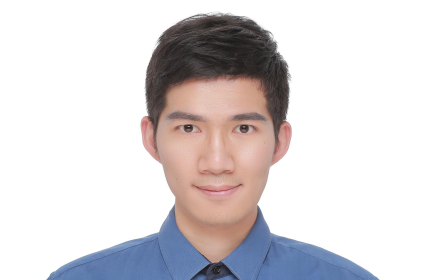
\includegraphics[height=2cm]{../people/xiaoyanxu}
  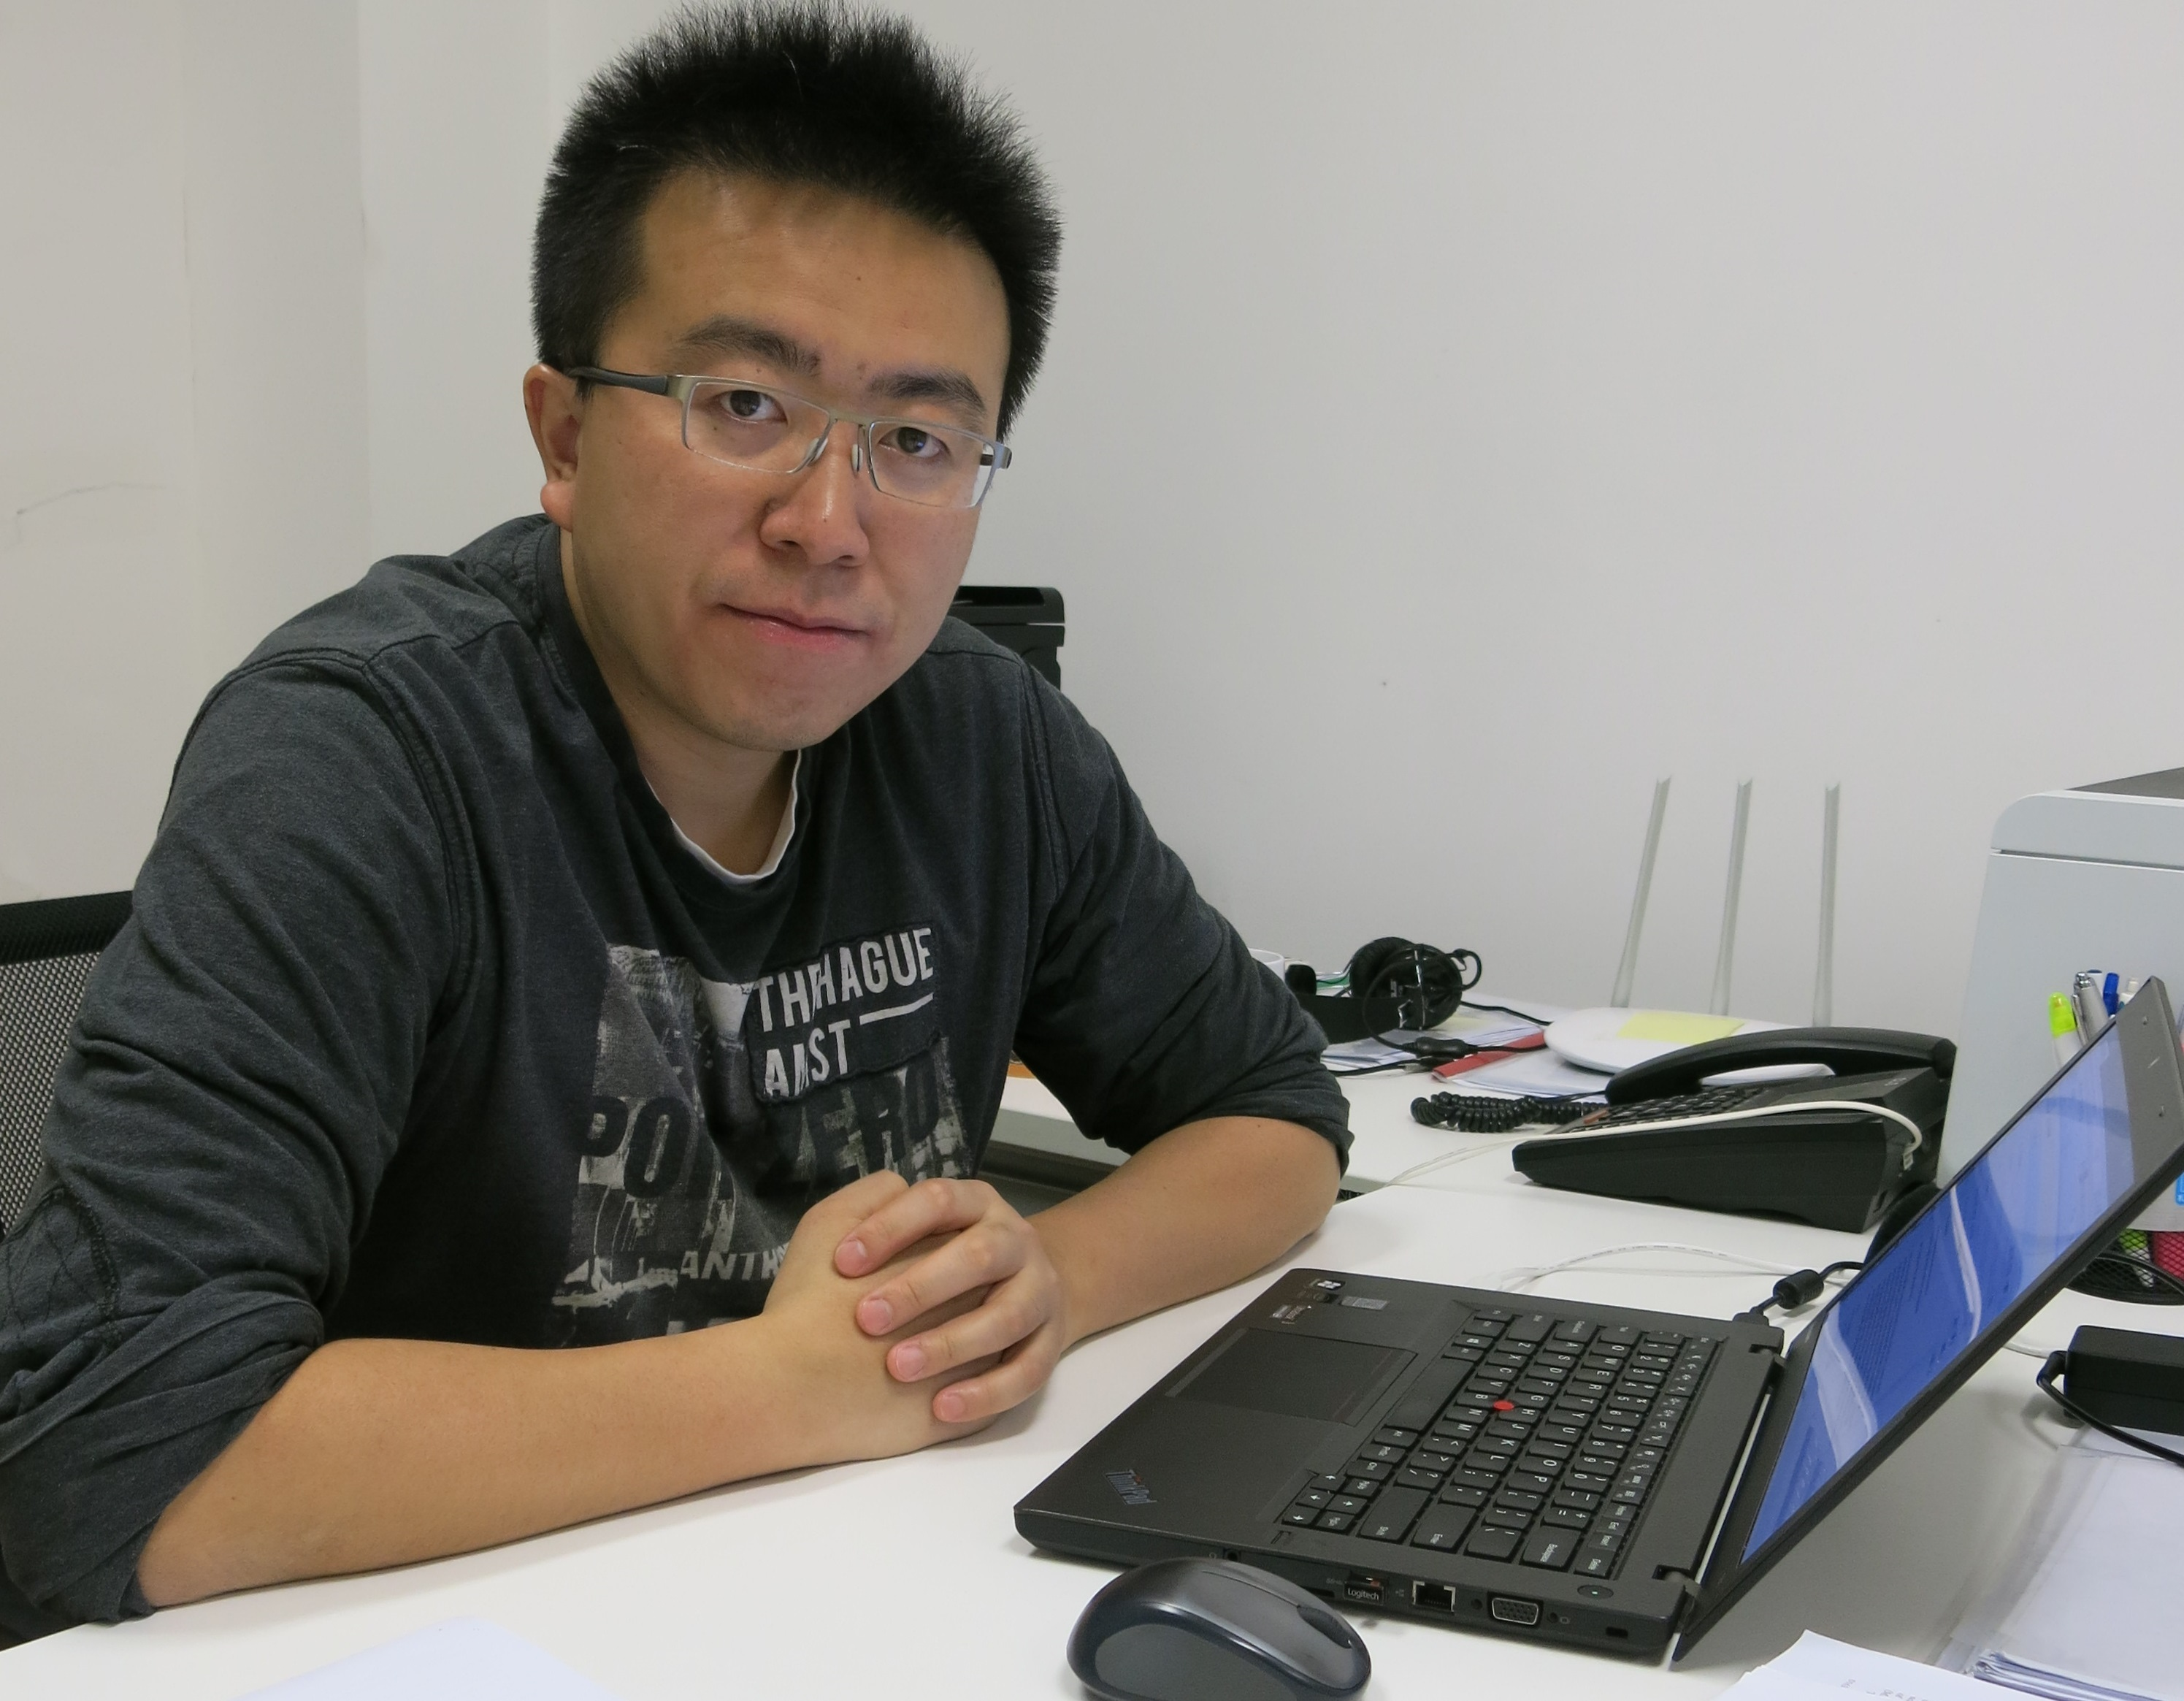
\includegraphics[height=2cm]{../people/ziyangmeng}\\
  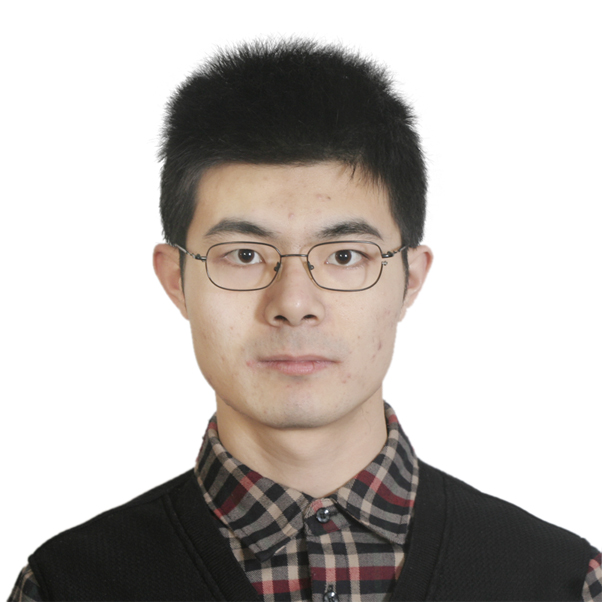
\includegraphics[height=2cm]{../people/zhanglong}
  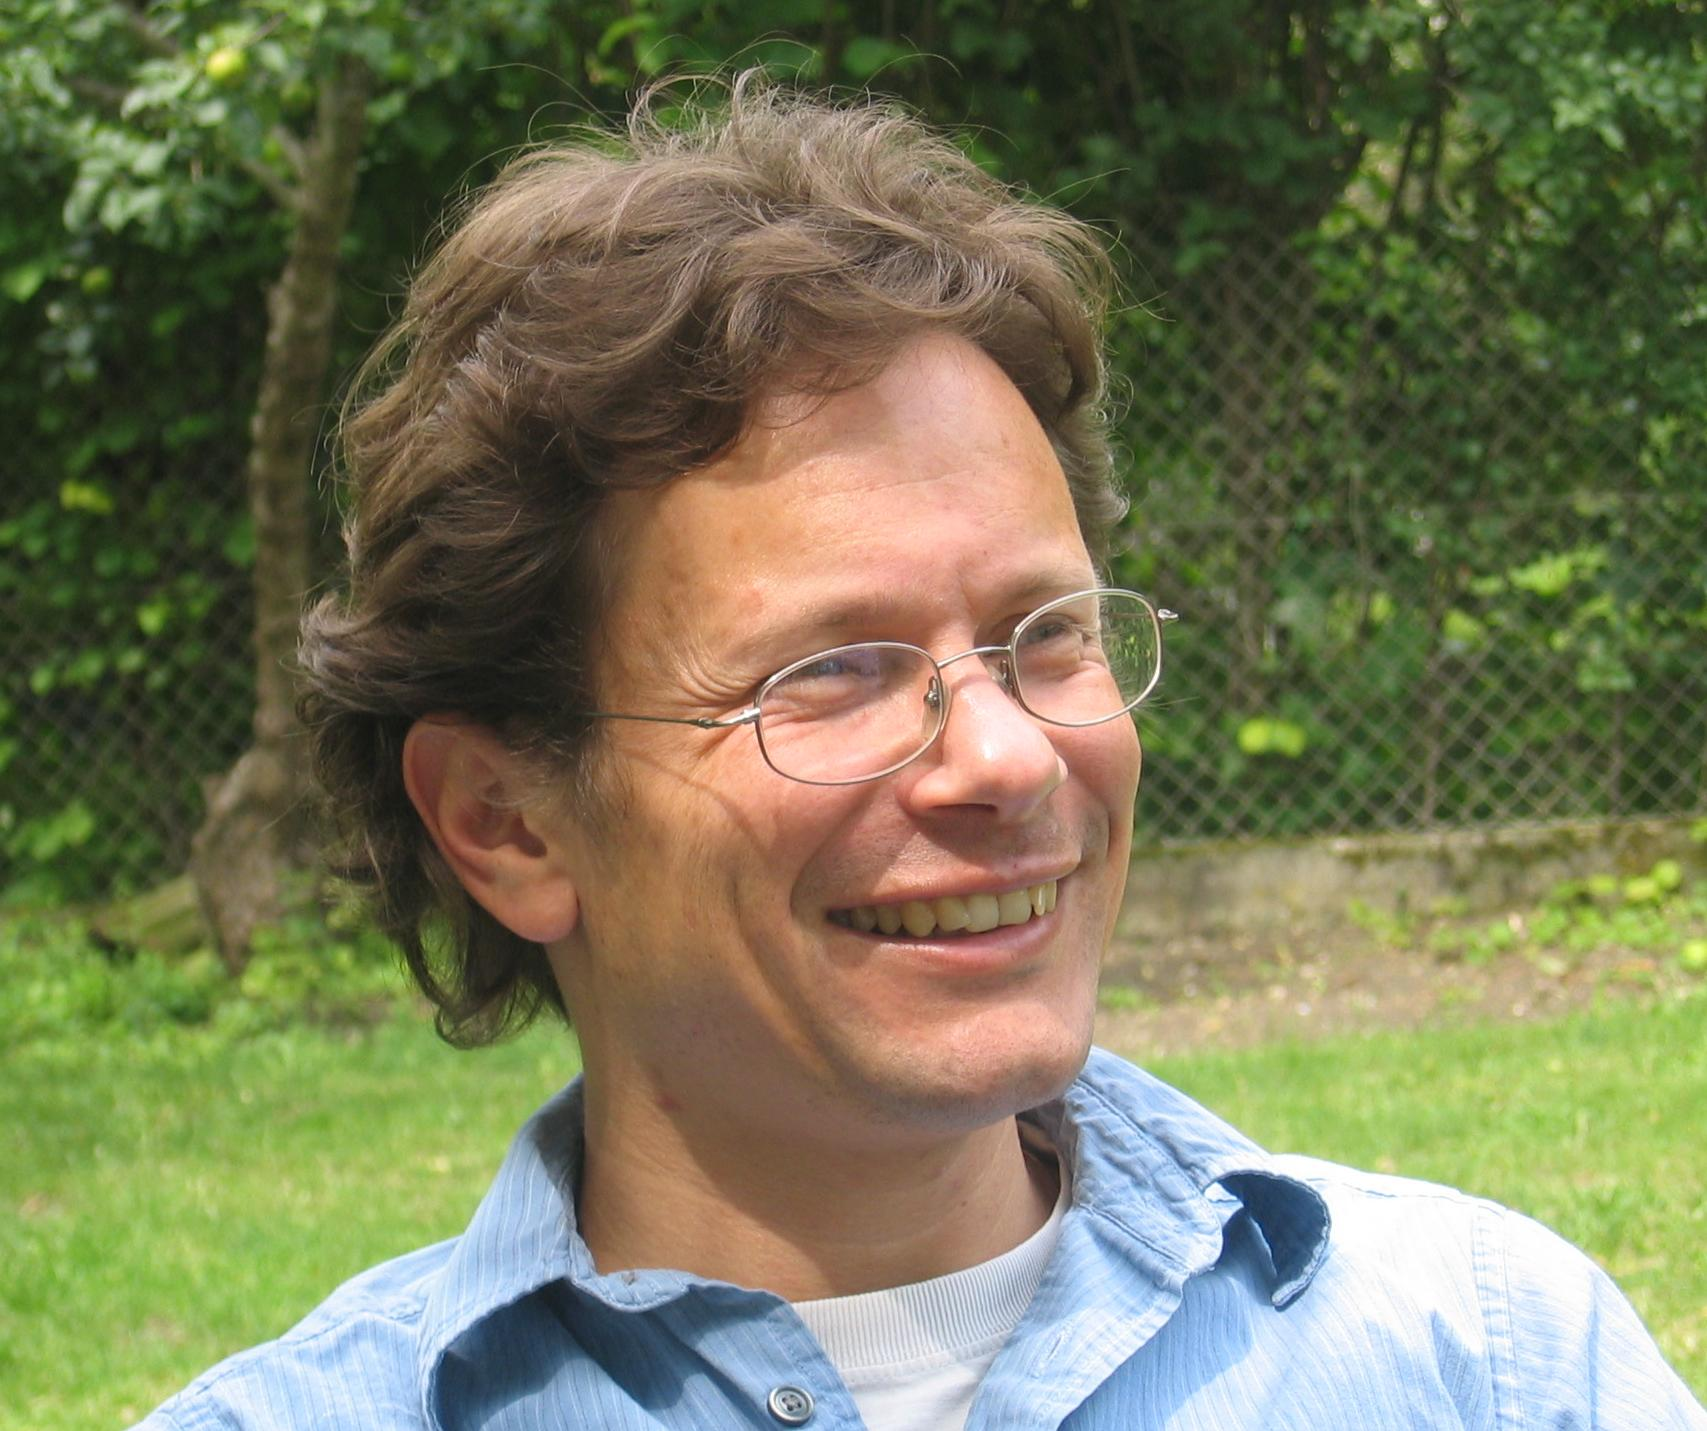
\includegraphics[height=2cm]{../people/fakher}
  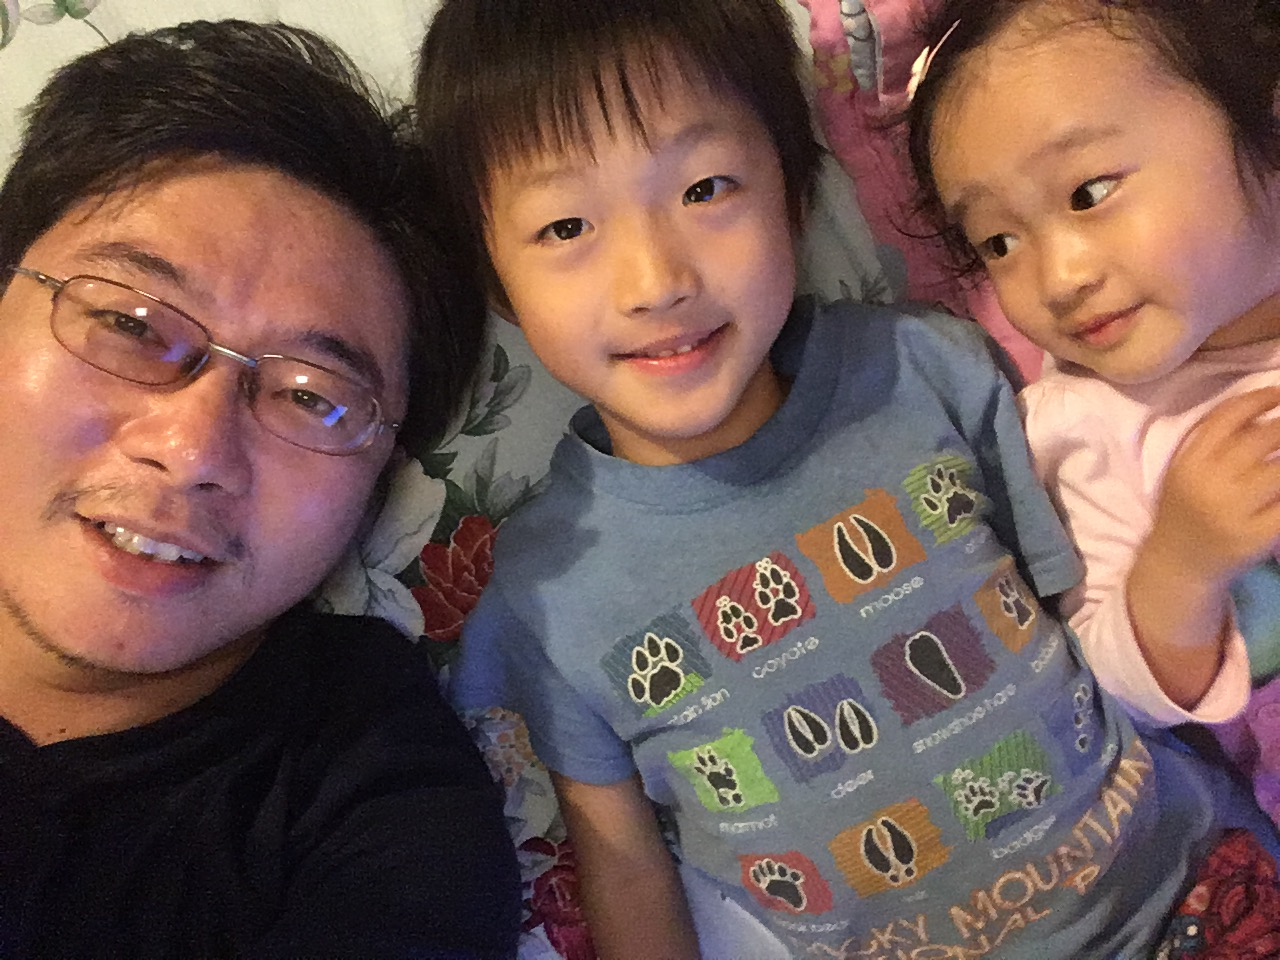
\includegraphics[height=2cm]{../people/cenke}
\end{center}
\end{itemize}
\begin{center}
  \small Phys. Rev. X \textbf{9}, 021022 (2019).
\end{center}
\end{frame}

\begin{frame}{Collaborators}
\begin{itemize}
\item Chuang Chen, Institute of Physics, CAS.
\item Xiao Yan Xu, Hong Kong University of Science and Technology.
\item Zi Yang Meng, Hong Kong University.
\begin{center}
  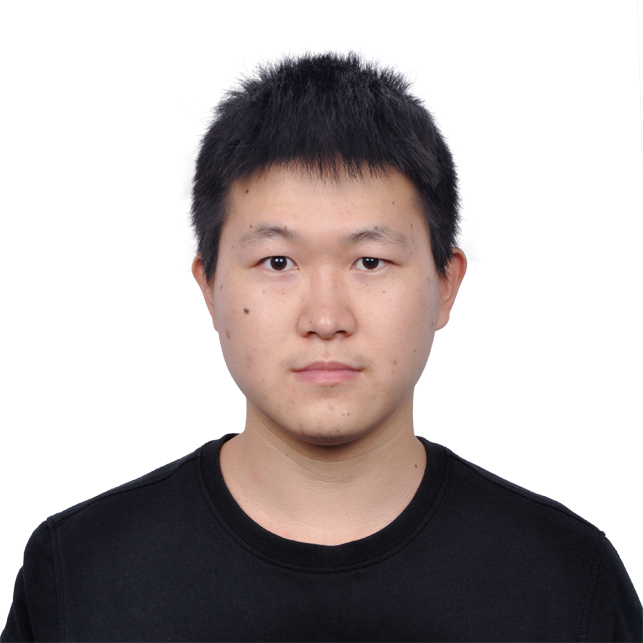
\includegraphics[height=2cm]{../people/chuangchen}
  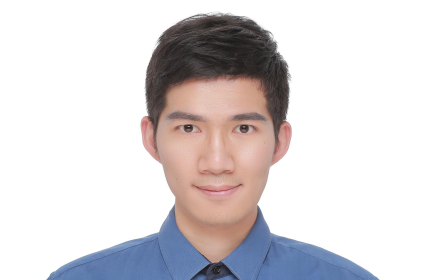
\includegraphics[height=2cm]{../people/xiaoyanxu}
  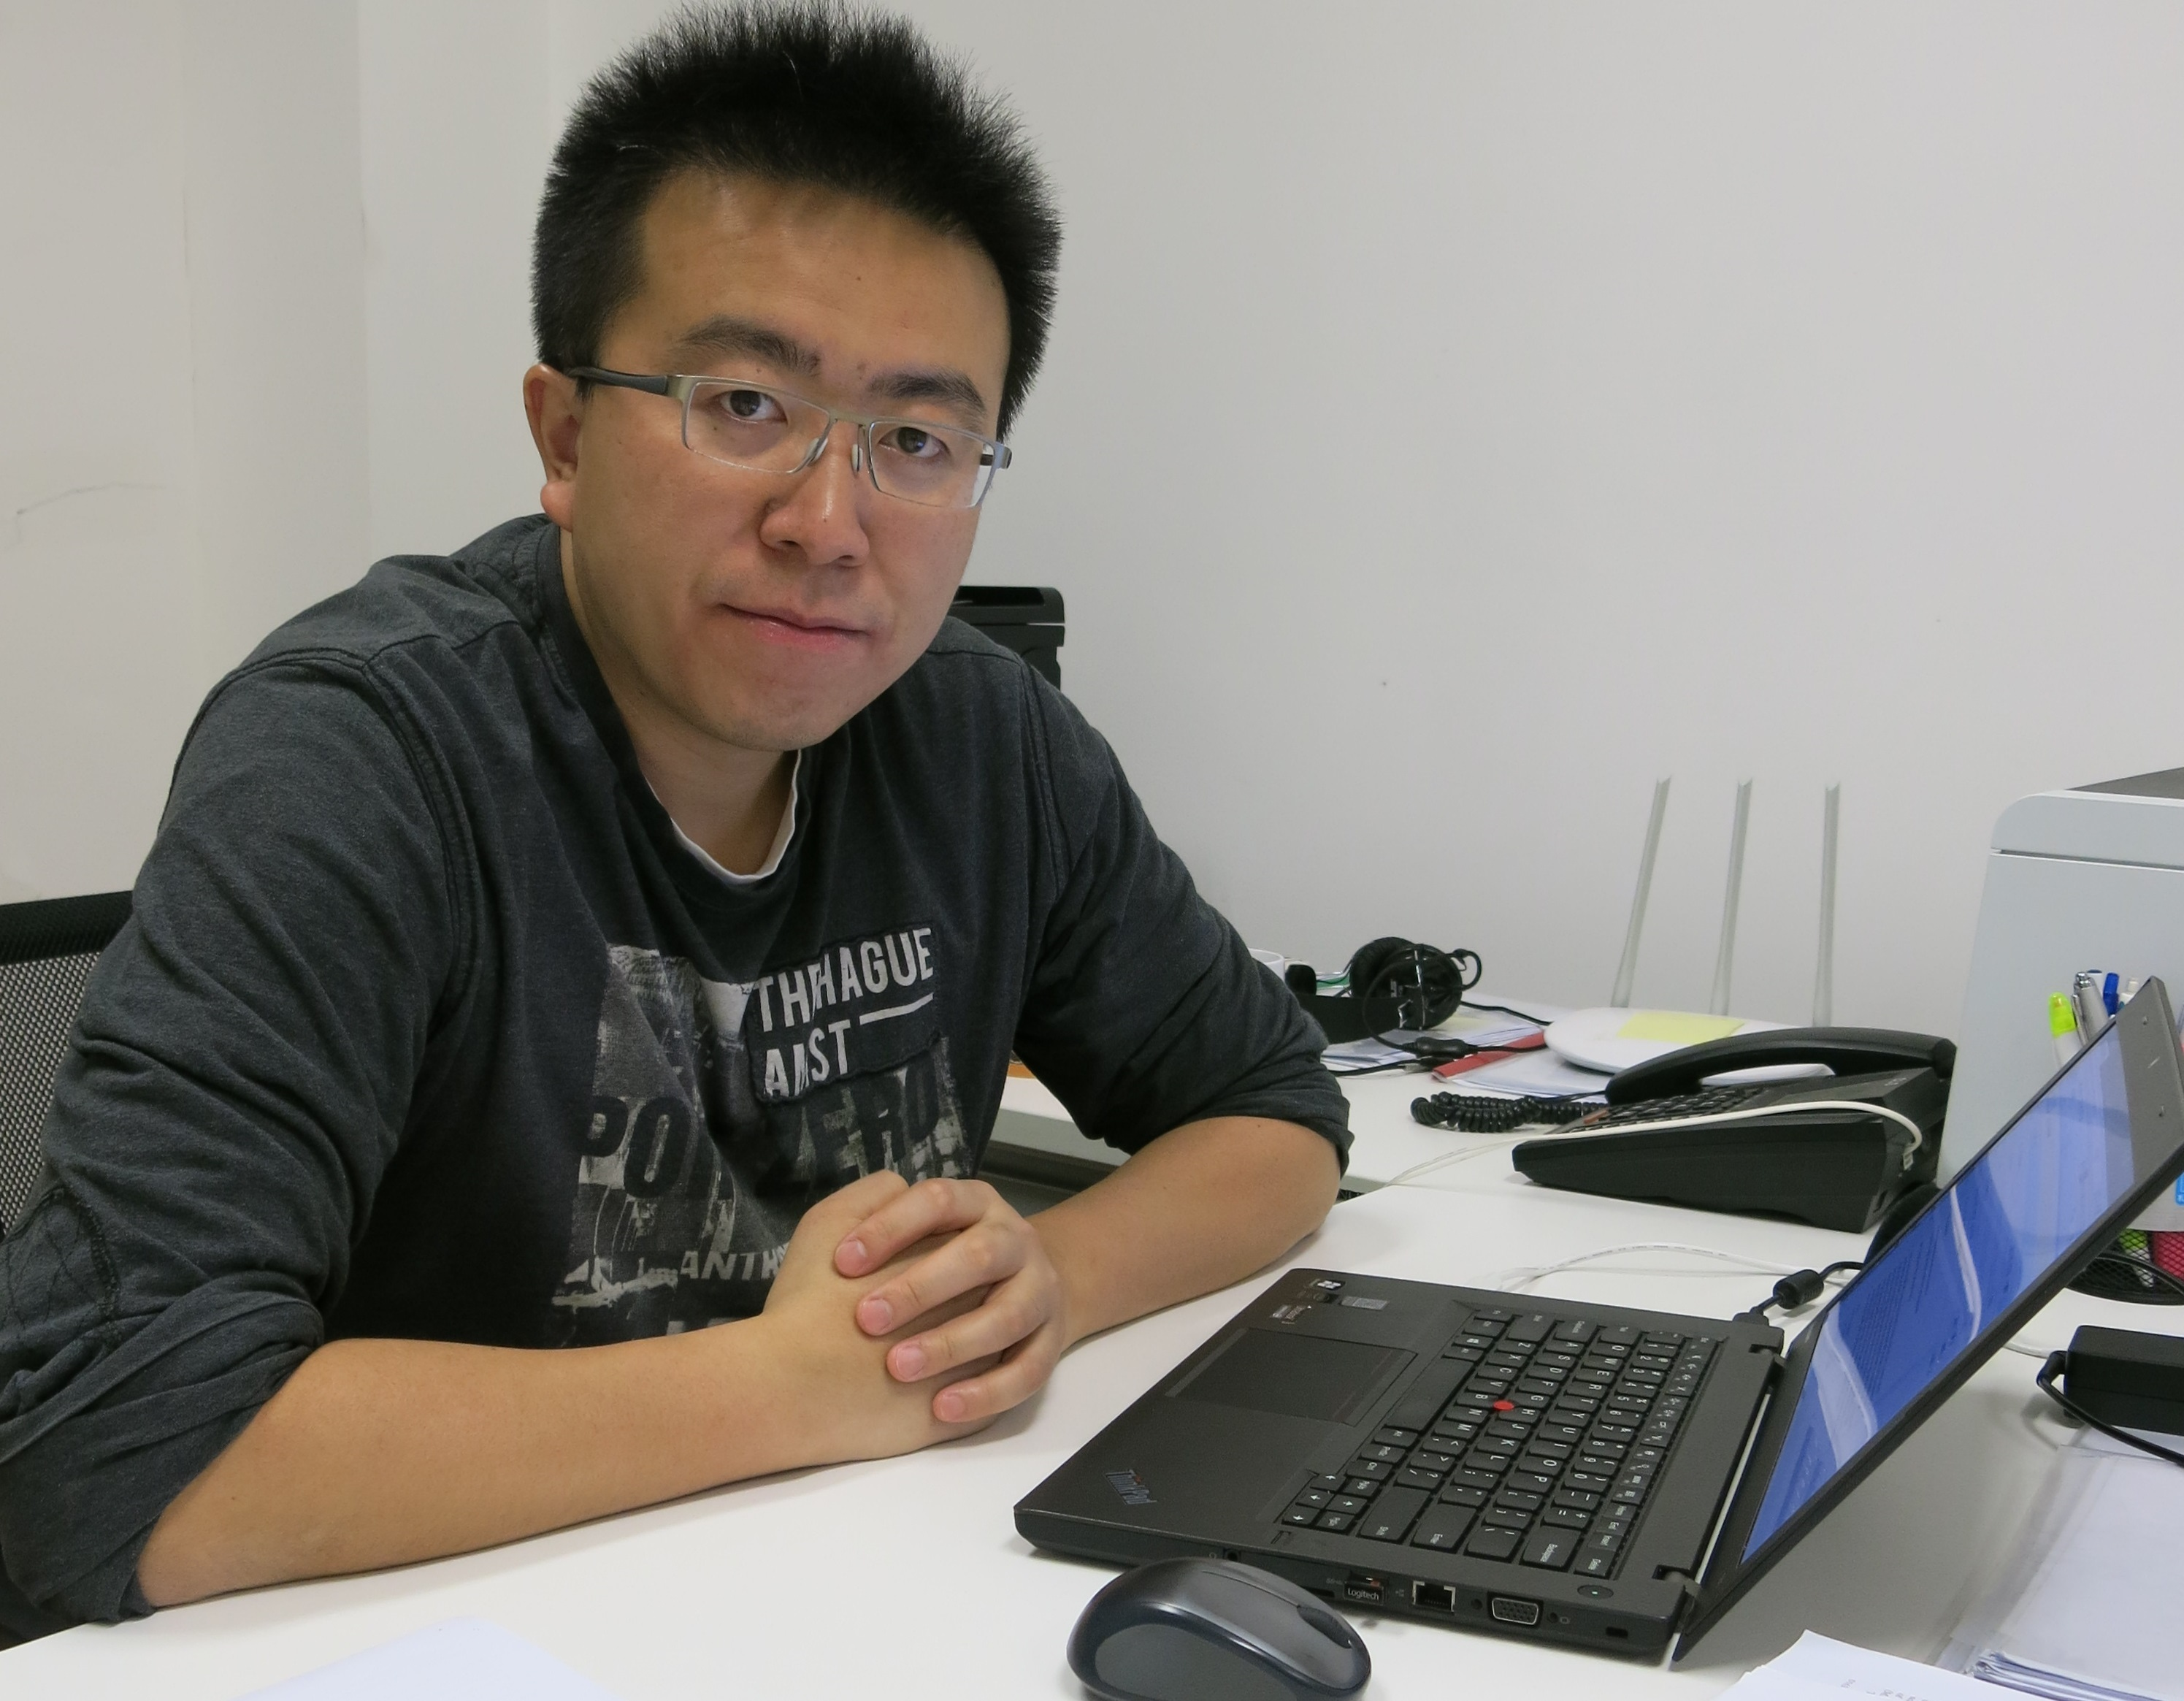
\includegraphics[height=2cm]{../people/ziyangmeng}
\end{center}
\end{itemize}
\begin{center}
  \small arXiv:1904.12872
\end{center}
\end{frame}

\begin{frame}{Outline}
	%\begin{columns}
	%\column{.7\textwidth}
		\tableofcontents
  %\end{columns}
  % You might wish to add the option [pausesections]
\end{frame}

\section{Introduction: DQMC and Designed Hamiltonians}

\begin{frame}
  \frametitle{The Determinant Quantum Monte Carlo Method}
  \begin{align*}
  L_F &= \sum_{\langle i,j \rangle\alpha}{\psi}^{\dagger}_{i\alpha} \left[(\partial_\tau -\mu)\delta_{ij}-t e^{i\phi_{ij}}   \right]   {\psi}_{j\alpha} + \text{h.c.}\\
  L_\phi &= \frac{4} {JN_{f}\Delta \tau ^2} \sum_{\langle i,j \rangle}
  \left[ 1-\cos(\phi_{ij}(\tau+1)-\phi_{ij}(\tau))
   +\frac{1}{2}K N_f\sum_{\square}\cos (\text{curl} \phi) \right],
\end{align*}
\begin{itemize}
  \item Sampling bosonic configuration: $\phi = \{\phi_{ij}(\tau)\}$.
  \item Weight:
  \[W[\phi] = W_b[\phi]\det(\mathbf I + \mathbf B(\beta,0;\phi))\]
  \item Complexity: $O(\beta N^3)$.
  \item Metropolis Algorithm and Fast Update:
  \[\phi_{ij}(\tau)\rightarrow\phi_{ij}(\tau)+\delta\phi;\quad p(\delta\phi)\propto e^{-\delta\phi^2/(2\Delta^2)}\].
\end{itemize}
\end{frame}

\begin{frame}
\frametitle{Designer Hamiltonians}
\begin{columns}
	\column{.6\textwidth}
	\begin{center}
		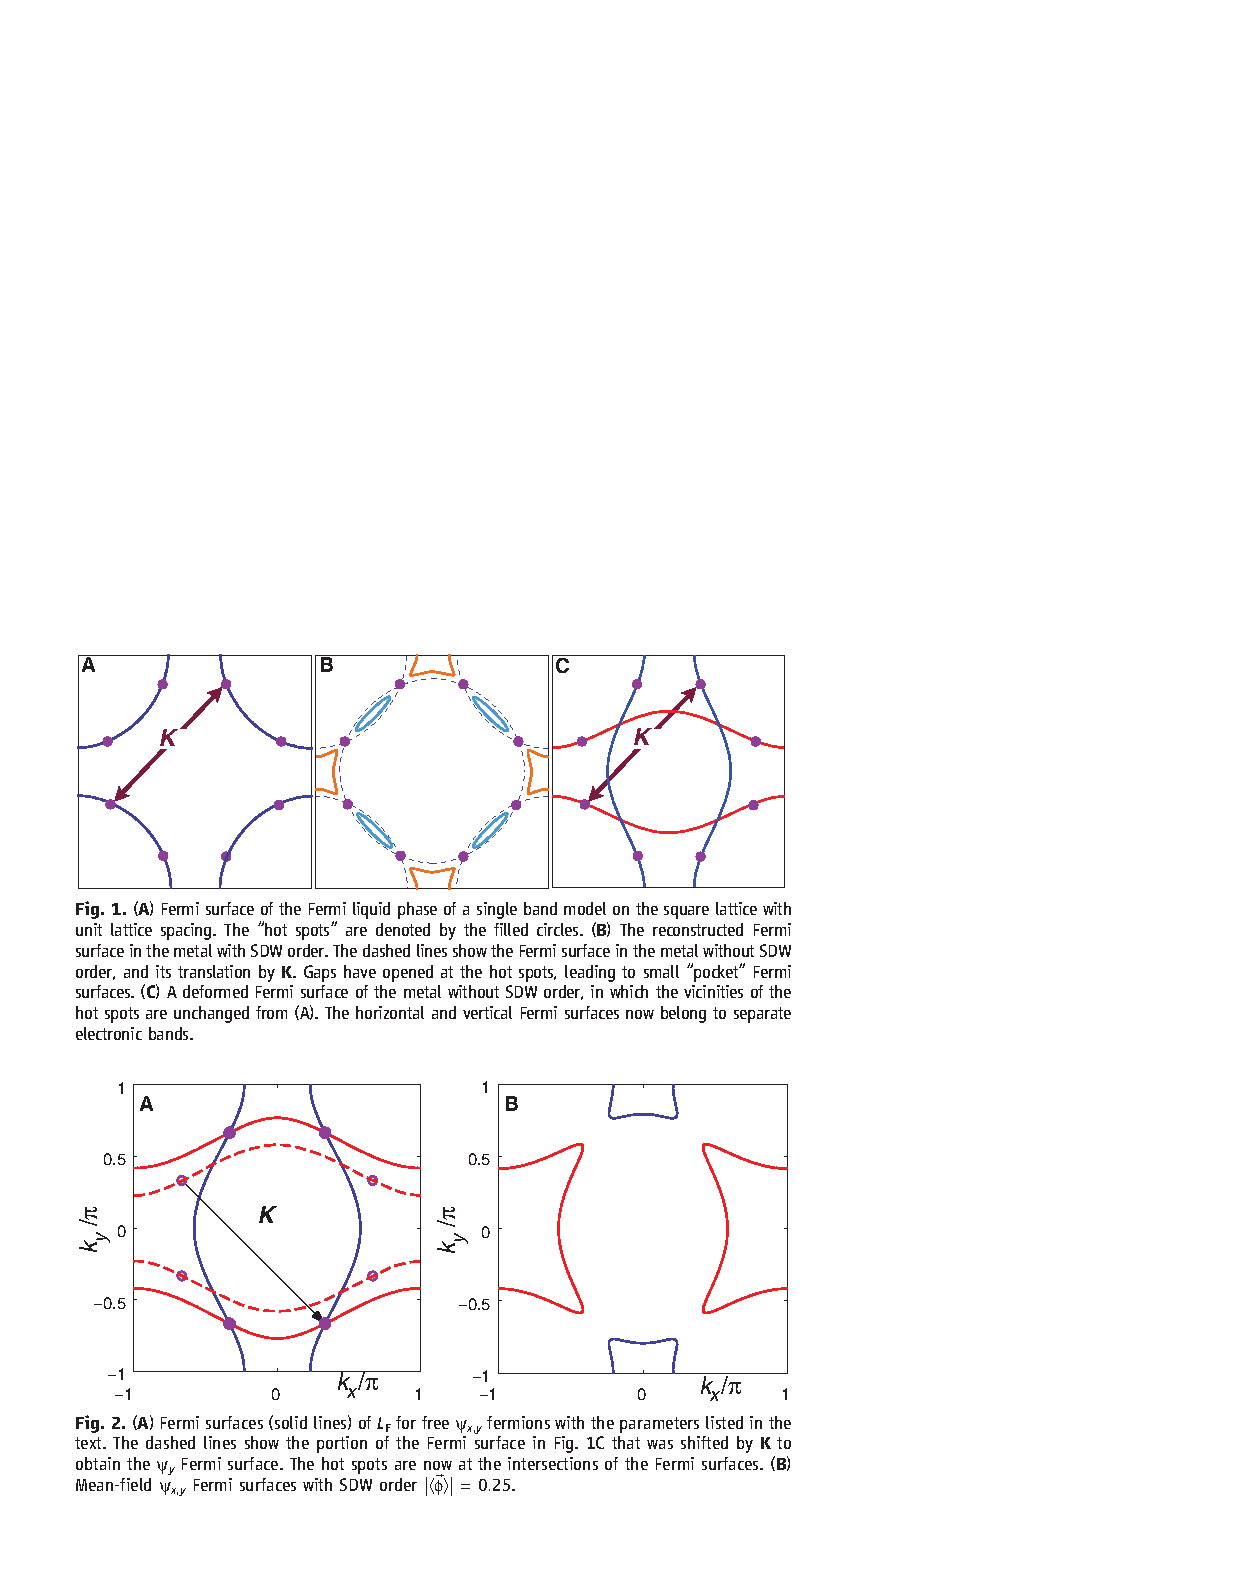
\includegraphics[width=\columnwidth]{../orthogonal_metal/berg2012}
	\end{center}
	\column{.4\textwidth}
	\begin{itemize}
		\item E Berg, M Metlitski and S Sachdev,\\ Science 2012.
		\item Use a two-band model to simulate SDW instability in cuprates.
		\item Two-band model removes sign problem.
	\end{itemize}
\end{columns}
\end{frame}

\begin{frame}
	\frametitle{Simulating effective models of spin liquids}
		\begin{center}
			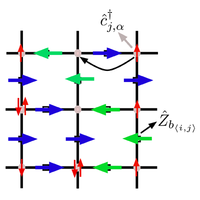
\includegraphics[width=4cm]{../orthogonal_metal/z2dsl}
		\end{center}
		\begin{itemize}
			\item F Assaad and T Grover, PRX 2016
			\item S Gazit, M Randeria and A Vishwanath, Nat Phys 2017
			\item Simulated $\mathbb Z_2$-Dirac spin liquid
		\end{itemize}
\end{frame}

\begin{frame}
	\frametitle{Questions to address}
	\begin{itemize}
		\item[\ding{51}] Realizing exotic states of matter in a Monte Carlo simulation.
		\item[\ding{51}] Universal properties at strongly-interacting IR: gapless phases or quantum critical points.
		\item[\ding{55}] Which realistic model realizes it?
		\item[\ding{55}] Which material realizes it?
	\end{itemize}

\end{frame}

\section{Example: U(1)-Dirac Quantum Spin Liquid}

\subsection{Introduction}

\begin{frame}
  \frametitle{U(1) Quantum Spin Liquid: History and Outlooks}
\begin{itemize}
	\item U(1)-Dirac spin liquid: Dirac-fermion spinons + U(1) gauge field.
	\[\mathcal L = \bar\psi_\alpha \gamma^\mu(\partial_\mu-iA_\mu)\psi +  F_{\mu\nu}^2,\quad
	\vec S_i = \psi^\dagger_{i\alpha}\vec\sigma_{\alpha\beta}\psi_{i\beta}.\]
	\item $\pi$-flux phase in high-$T_c$ cuprates:\\
	\emph{\small I. Affleck and J. B. Marston, Phys. Rev. B 37, 3774 (1988).}
	\item Spin liquid in frustrated magnets: kagome-lattice Heisenberg model?\\
	\emph{\small Y. Ran, M. Hermele, P. A. Lee, and X.-G. Wen, Phys. Rev. Lett. 98, 117205 (2007).}

  \item Does the mean-field picture stand: Is the U(1) gauge field deconfined?
\end{itemize}
\end{frame}

%\begin{frame}
%  \frametitle{Compact U(1): Monopoles}
%  \begin{itemize}
%    \item Gauge theory in the continuum:
%    \[S=\int d^3x (\epsilon_{abc}A_c)^2.\]
%    \item Gauge theory on a lattice:
%    \[S=\sum_{\square}e^{iA_{ij}}e^{iA_{jk}}e^{iA_{kl}}e^{iA_{li}}.\]
%    \item Compact U(1) gauge connection: $A_{ij}\simeq A_{ij}+2\pi$.
%    \item Monopole: non-smooth space-time configurations of $A_{ij}$.
%    \item Even without matter field, compact U(1) is not free Maxwell theory: confinement in the IR.
%  \end{itemize}
%\end{frame}

\begin{frame}
	\frametitle{Does U(1) spin liquid exist in 2+1D?}
	\[\mathcal L = \bar\psi_\alpha \gamma^\mu(\partial_\mu-iA_\mu)\psi + F_{\mu\nu}^2.\]
	\begin{itemize}
		\item U(1) monopole: confinement. Compact U(1) is \alert{not free}.
		\item Gapless fermions suppress monopole.
	\end{itemize}
	\begin{tabular}{p{.3\textwidth}p{.3\textwidth}p{.3\textwidth}}
		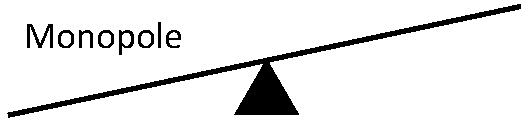
\includegraphics[scale=.35]{../u1sl/balance1}
		&
		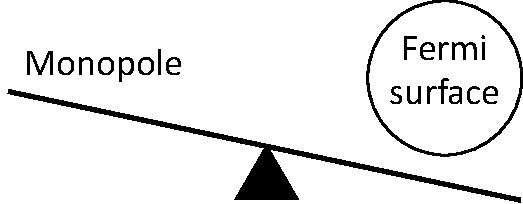
\includegraphics[scale=.35]{../u1sl/balance2}
		&
		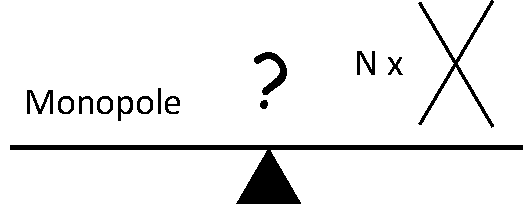
\includegraphics[scale=.35]{../u1sl/balance3}\\
		Pure compact U(1). & Spinon FS. & A critical $N_f$?\\
		Polyakov, Gauge fields and strings. & Sung-Sik Lee, PRB 78 085129 (2008). & Under heavy debate: large-$N_f$ expansion / CFT argument / numerical simulations.
	\end{tabular}
\end{frame}

\subsection{Model and Method}

\begin{frame}
  \frametitle{The Model Hamiltonian}
  \[
  H=\frac{1}{2}JN_{f}\sum_{\langle i,j \rangle} \frac 1 4 \hat{L}^{2}_{ij}-t\sum_{\langle i,j \rangle\alpha}\left(\hat{c}^{\dagger}_{i\alpha}e^{i\hat{\theta}_{ij}}\hat{c}_{j\alpha}+\text{h.c.}\right)
  +\ \frac{1}{2}K\ N_f\sum_{\square}\cos \left( \text{curl} \hat{\theta} \right).
\]
\begin{columns}
  \column{.8\textwidth}
  \begin{itemize}
    \item $c$: spinon.
    \item $\theta_{ij}$: quantum rotors $\Rightarrow$ compact gauge field.
    \item $[L_{ij}, e^{i\theta_{ij}}]=e^{i\theta_{ij}}$ is the angular momentum / electric field.
    \item Gauge symmetry:
    \[\hat{Q}_{i} = -\sum_{j}\hat{L}_{ij} + \sum_{\alpha} \left( \hat{c}^{\dagger}_{i\alpha}\hat{c}^{\phantom\dagger}_{i\alpha} - 1/2 \right);[H, \hat Q_i] = 0.\]
    \item Dynamically generated constraint:
		$\hat Q_i \simeq 0$ implies gauge symmetry.
    \item $K>0$ favors a $\pi$-flux state.
		\item $N_f=1$: two Dirac cones (two valley). $N_f=2,4,6,\ldots$ do not have sign problem.
  \end{itemize}

  \column{.2\textwidth}
  \begin{center}
    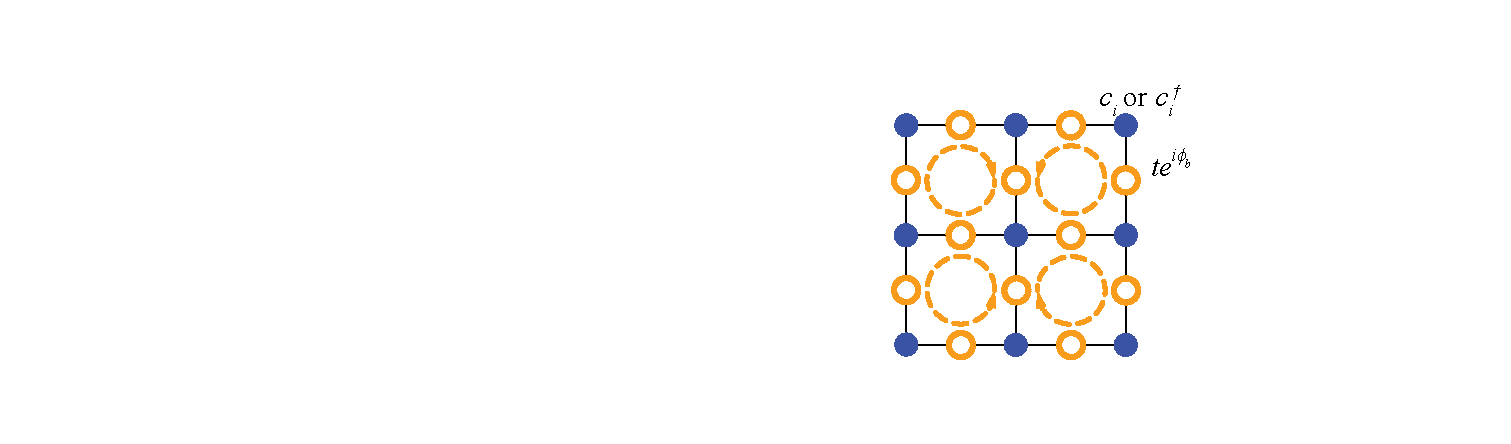
\includegraphics[width=3cm]{../u1sl/model}
  \end{center}
\end{columns}
\end{frame}

\subsection{Results}

\begin{frame}
  \frametitle{Phase diagrams}
  \begin{center}
    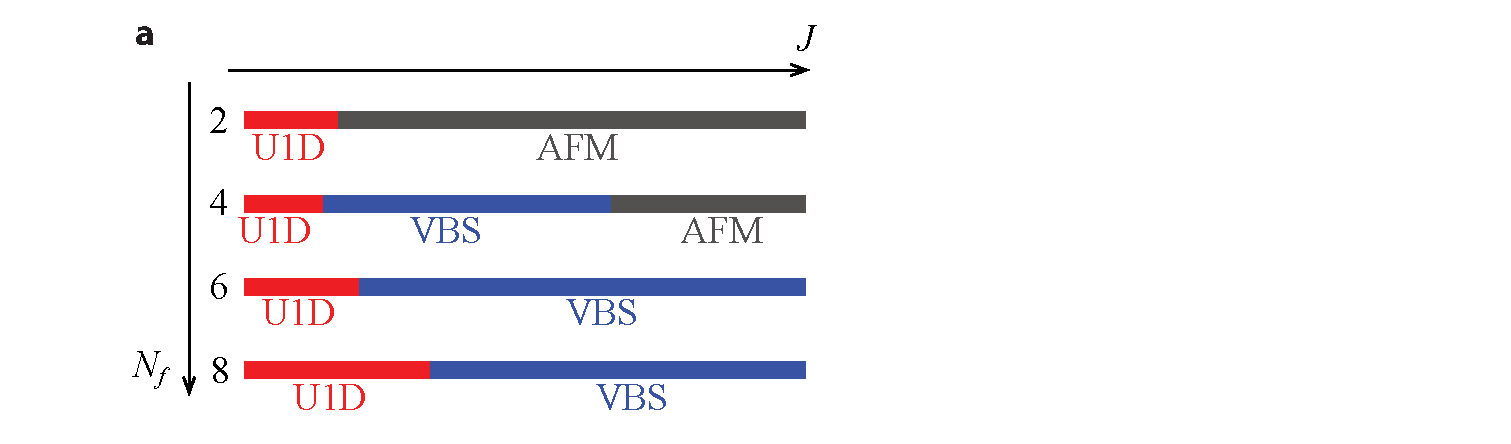
\includegraphics[width=5cm]{../u1sl/phase-diagram}
  \end{center}
  \begin{columns}[t]
    \column{.5\textwidth}
    \begin{block}{U(1)-Dirac Spin Liquid}
      \begin{itemize}
        \item Deconfined U(1) gauge field.
        \item Power-law spin-spin and dimer-dimer correlation functions.
        \item Algebraic spin liquid.
      \end{itemize}
    \end{block}

    \column{.5\textwidth}
    \begin{block}{Confinement phases}
      \begin{itemize}
        \item VBS or AFM long-range order.
        \item Fermion gapped.
        \item Confined U(1) gauge field.
      \end{itemize}
    \end{block}
  \end{columns}
\end{frame}

\begin{frame}
  \frametitle{$N_f=2$: phase boundary}
  \begin{columns}
		\column{.7\textwidth}
    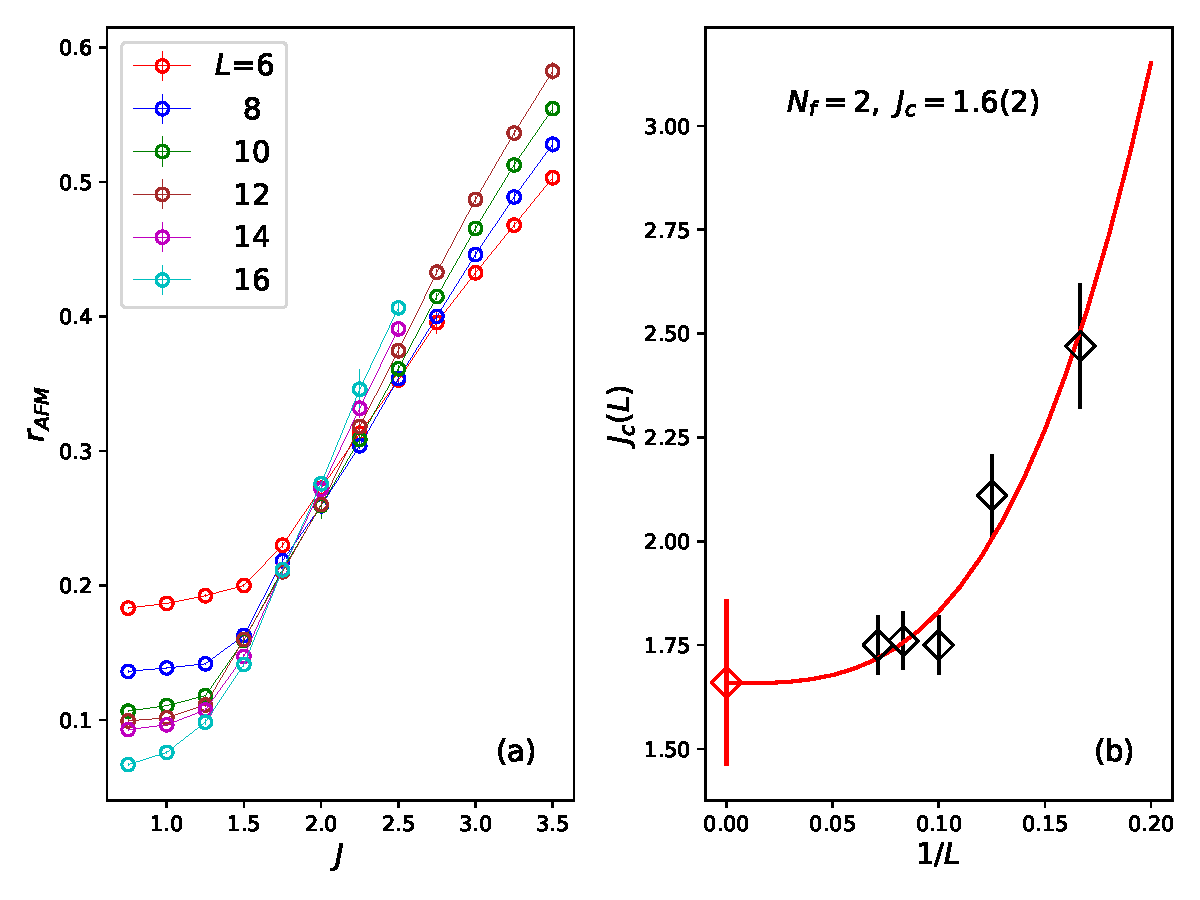
\includegraphics[width=\textwidth]{../u1sl/n2rafm}
		\column{.3\textwidth}
		\begin{itemize}
			\item Correlation ratio: $r = 1-\frac{\chi(\bm Q+\delta\bm q)}{\chi(\bm Q)}.$
			\item Crossing indicates the position of phase transition.
			\item Phase transition b/w U1D and AFM: $J_c=1.6(2)$.
		\end{itemize}
  \end{columns}
\end{frame}

\begin{frame}
  \frametitle{Deconfined U(1) gauge field}
  \begin{columns}
		\column{.6\textwidth}
    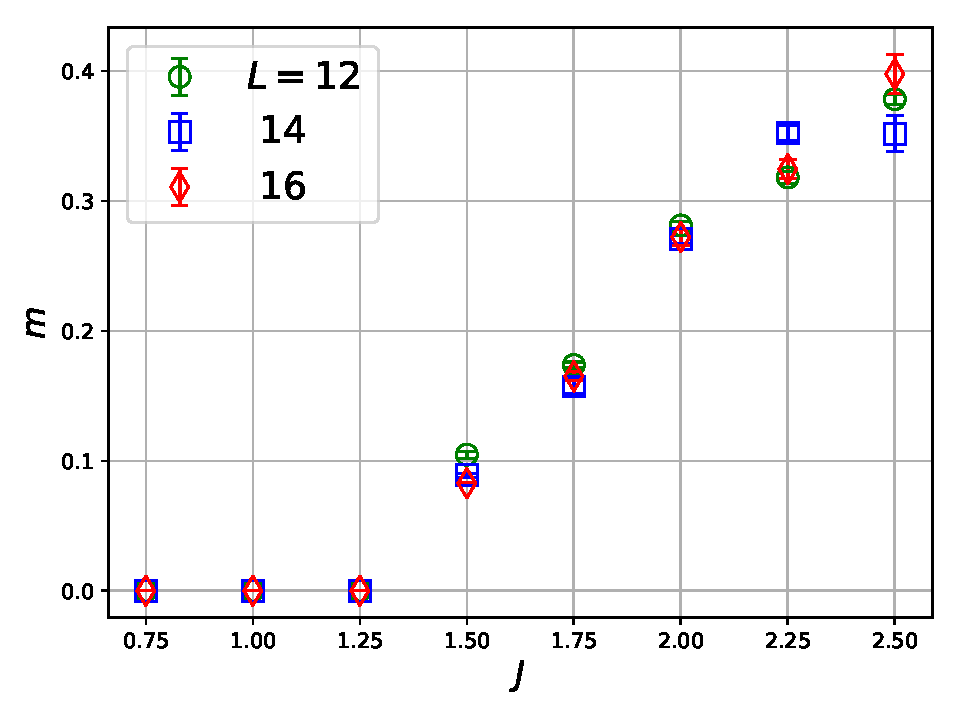
\includegraphics[width=\textwidth]{../u1sl/photonmass}
		\column{.4\textwidth}
		\begin{itemize}
			\item Measure photon mass $m$ from decaying of gauge-flux correlation functions.
			\item $m > 0$: confinement phase.
		\end{itemize}
  \end{columns}
\end{frame}

\begin{frame}
  \frametitle{$N_f=2$: U1D phase}
  \begin{columns}
		\column{.5\textwidth}
    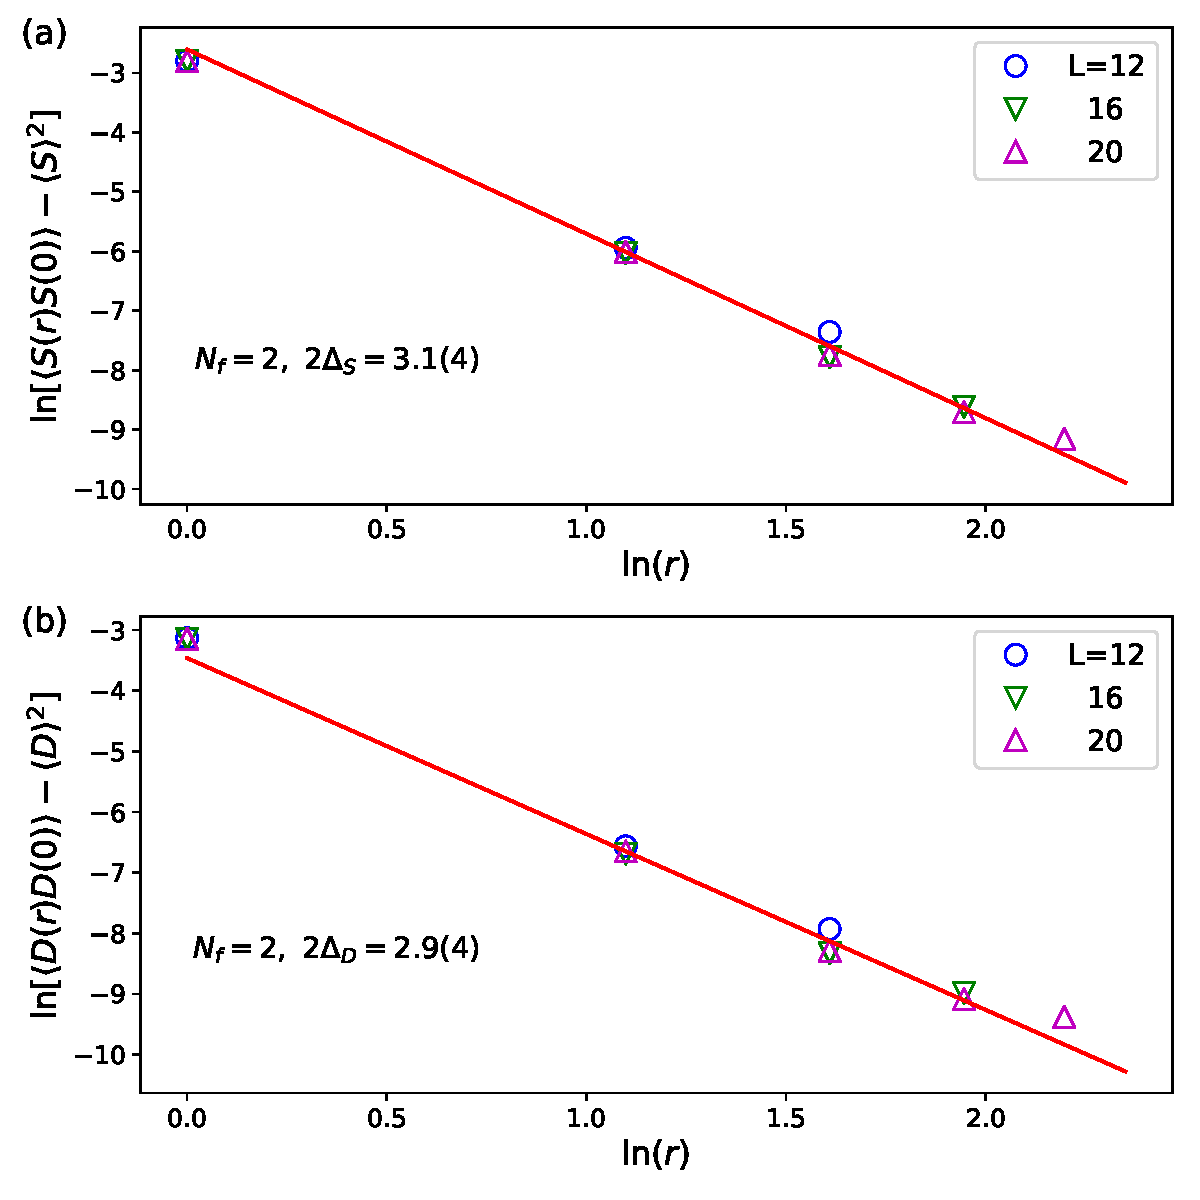
\includegraphics[width=\textwidth]{../u1sl/n2decay}
		\column{.5\textwidth}
		\begin{itemize}
			\item Spin and dimer OPs are fermion bilinears:
			\[\vec S = \psi^\dagger_{i\alpha}\vec\sigma_{\alpha\beta}\psi_{i\beta},\]
			\[D_{x,y} = \psi^\dagger_{i\alpha}\psi_{i+x,y,\beta}.\]
			\item Algebraic spin liquid: $\Delta_S = \Delta_D$.
		  \item (Free fermion has $\Delta_S=\Delta_D = 4$.)
		\end{itemize}
  \end{columns}
\end{frame}

\begin{frame}
  \frametitle{$N_f=4$: phase boundary}
  \begin{columns}
		\column{.7\textwidth}
    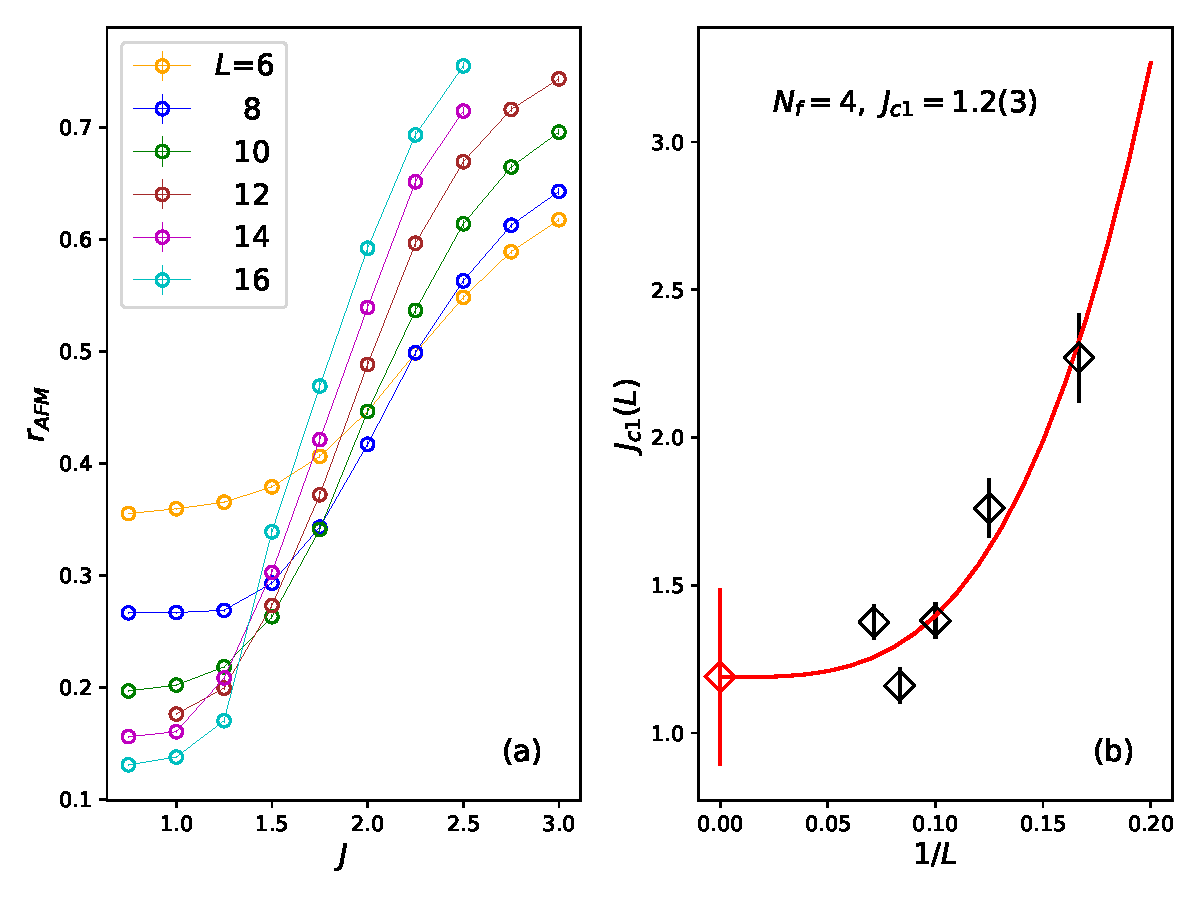
\includegraphics[width=\textwidth]{../u1sl/n4rvbs}
		\column{.3\textwidth}
		\begin{itemize}
			\item Phase transition b/w U1D and VBS: $J_c=1.2(3)$.
		\end{itemize}
  \end{columns}
\end{frame}

\begin{frame}
  \frametitle{$N_f=4$: U1D phase}
  \begin{columns}
		\column{.5\textwidth}
    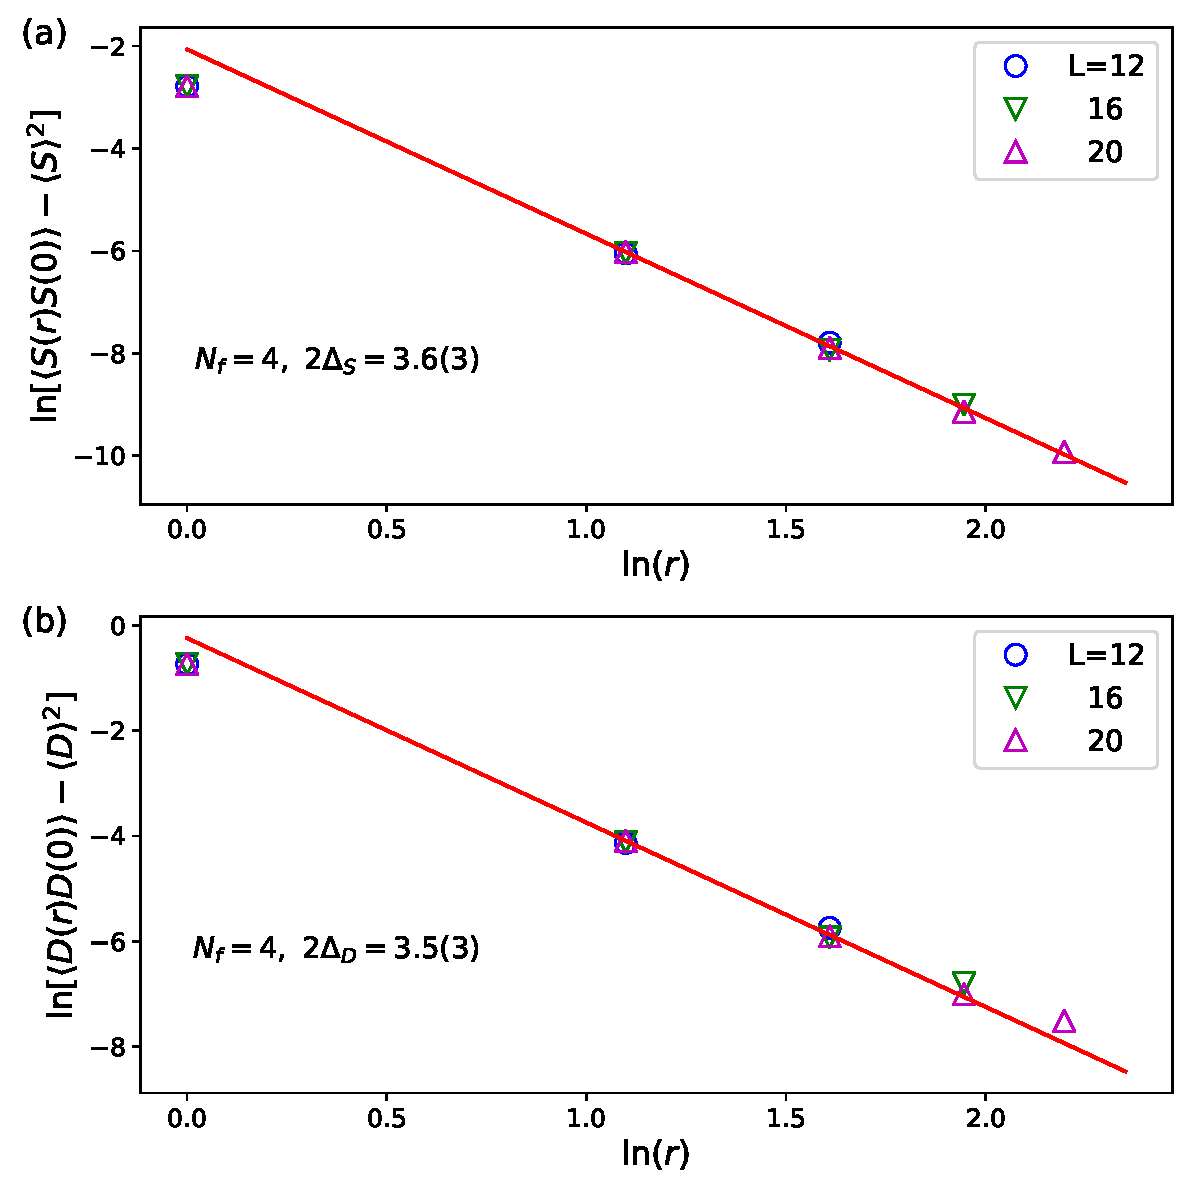
\includegraphics[width=\textwidth]{../u1sl/n4decay}
		\column{.5\textwidth}
		\begin{itemize}
			\item Spin and dimer OPs are fermion bilinears:
			\[\vec S = \psi^\dagger_{i\alpha}\vec\sigma_{\alpha\beta}\psi_{i\beta},\]
			\[D_{x,y} = \psi^\dagger_{i\alpha}\psi_{i+x,y,\beta}.\]
			\item Algebraic spin liquid: $\Delta_S = \Delta_D$.
		  \item (Free fermion has $\Delta_S=\Delta_D = 4$.)
		\end{itemize}
  \end{columns}
\end{frame}

\begin{frame}
  \frametitle{$N_f=6$: phase boundary}
  \begin{columns}
		\column{.7\textwidth}
    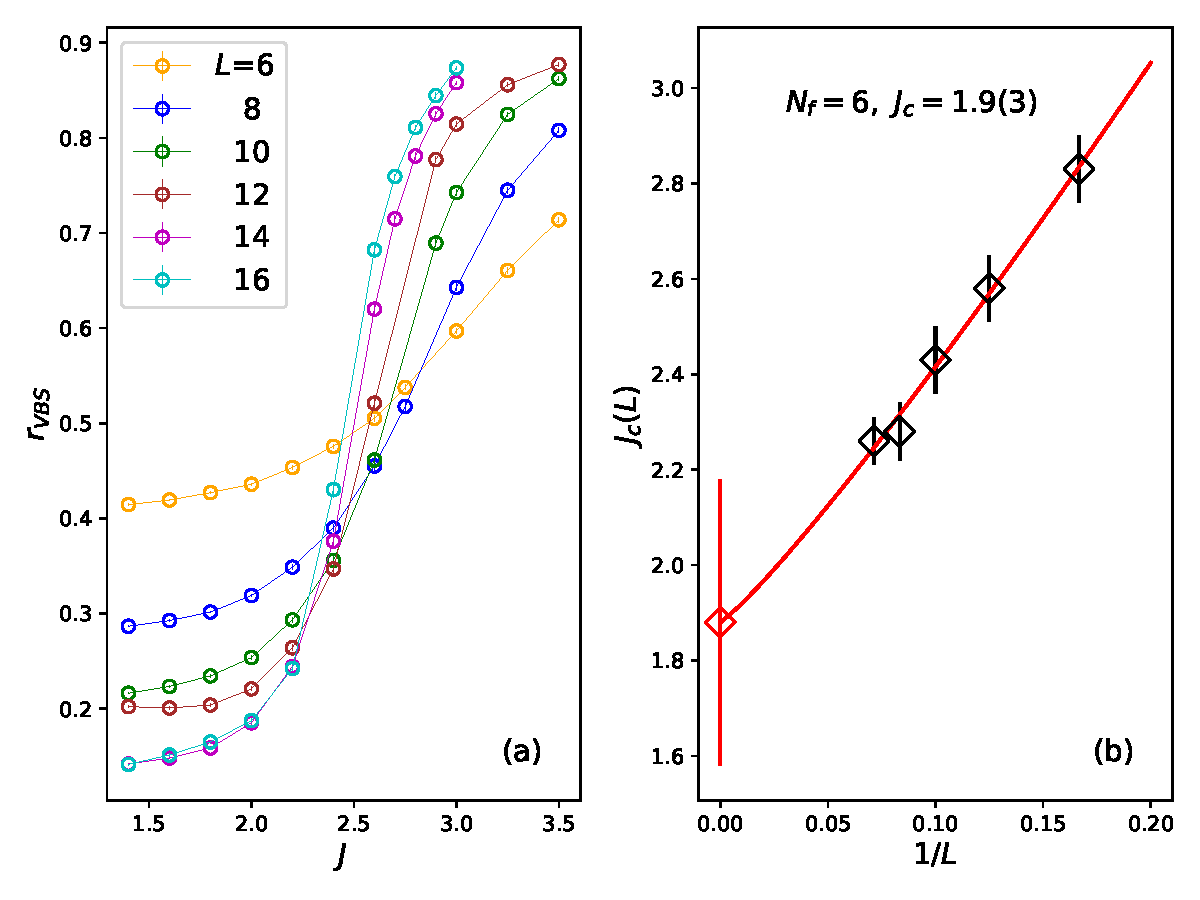
\includegraphics[width=\textwidth]{../u1sl/n6rvbs}
		\column{.3\textwidth}
		\begin{itemize}
			\item Phase transition b/w U1D and VBS: $J_c=1.9(3)$.
		\end{itemize}
  \end{columns}
\end{frame}

\begin{frame}
  \frametitle{$N_f=6$: U1D phase}
  \begin{columns}
		\column{.5\textwidth}
    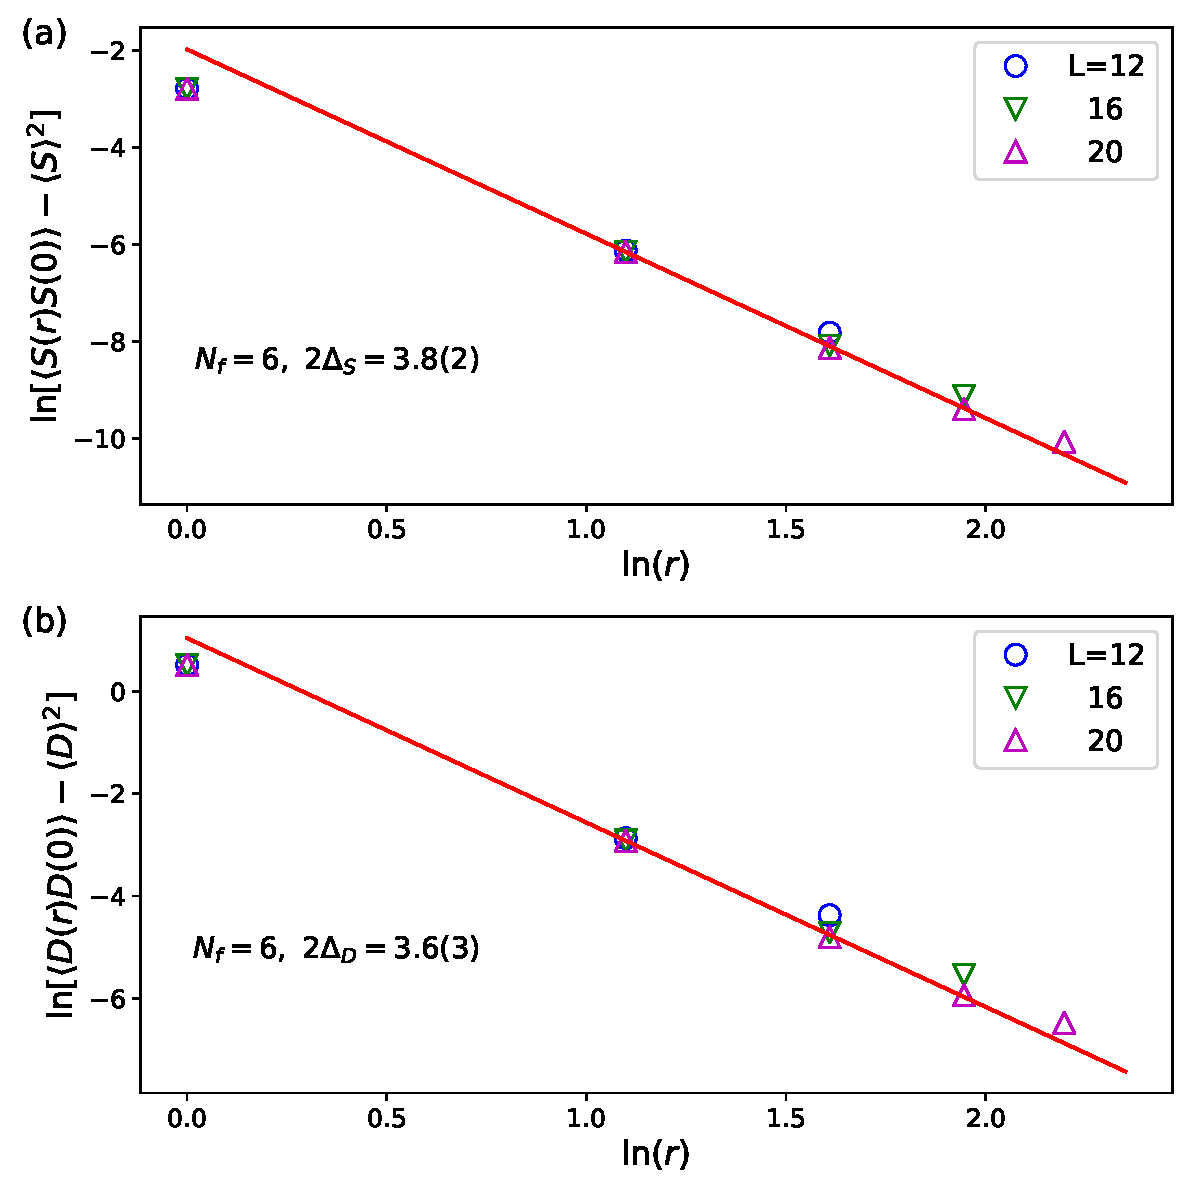
\includegraphics[width=\textwidth]{../u1sl/n6decay}
		\column{.5\textwidth}
		\begin{itemize}
			\item Spin and dimer OPs are fermion bilinears:
			\[\vec S = \psi^\dagger_{i\alpha}\vec\sigma_{\alpha\beta}\psi_{i\beta},\]
			\[D_{x,y} = \psi^\dagger_{i\alpha}\psi_{i+x,y,\beta}.\]
			\item Algebraic spin liquid: $\Delta_S = \Delta_D$.
		  \item (Free fermion has $\Delta_S=\Delta_D = 4$.)
		\end{itemize}
  \end{columns}
\end{frame}

\begin{frame}
  \frametitle{$N_f=8$: phase boundary}
  \begin{columns}
		\column{.7\textwidth}
    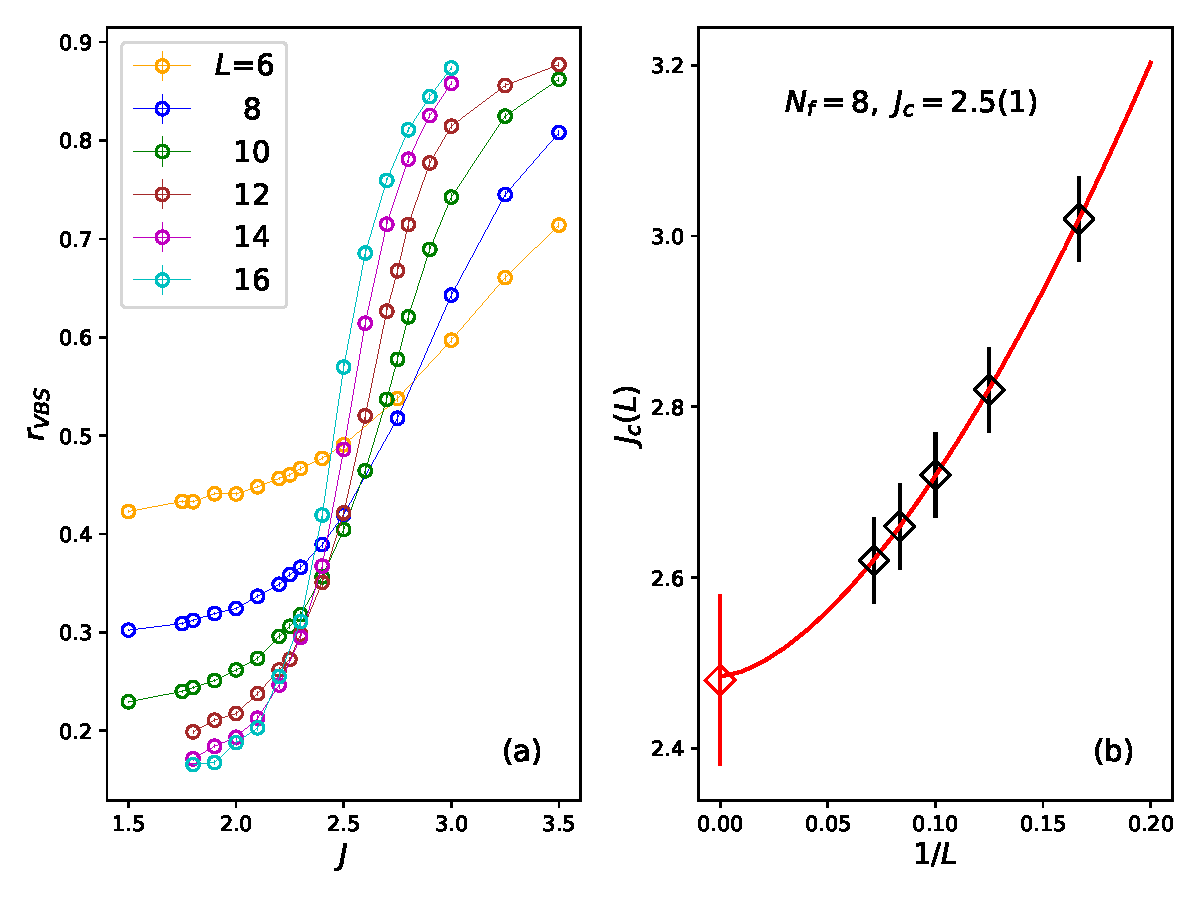
\includegraphics[width=\textwidth]{../u1sl/n8rvbs}
		\column{.3\textwidth}
		\begin{itemize}
			\item Phase transition b/w U1D and VBS: $J_c=2.5(1)$.
		\end{itemize}
  \end{columns}
\end{frame}

\begin{frame}
  \frametitle{$N_f=8$: U1D phase}
  \begin{columns}
		\column{.5\textwidth}
    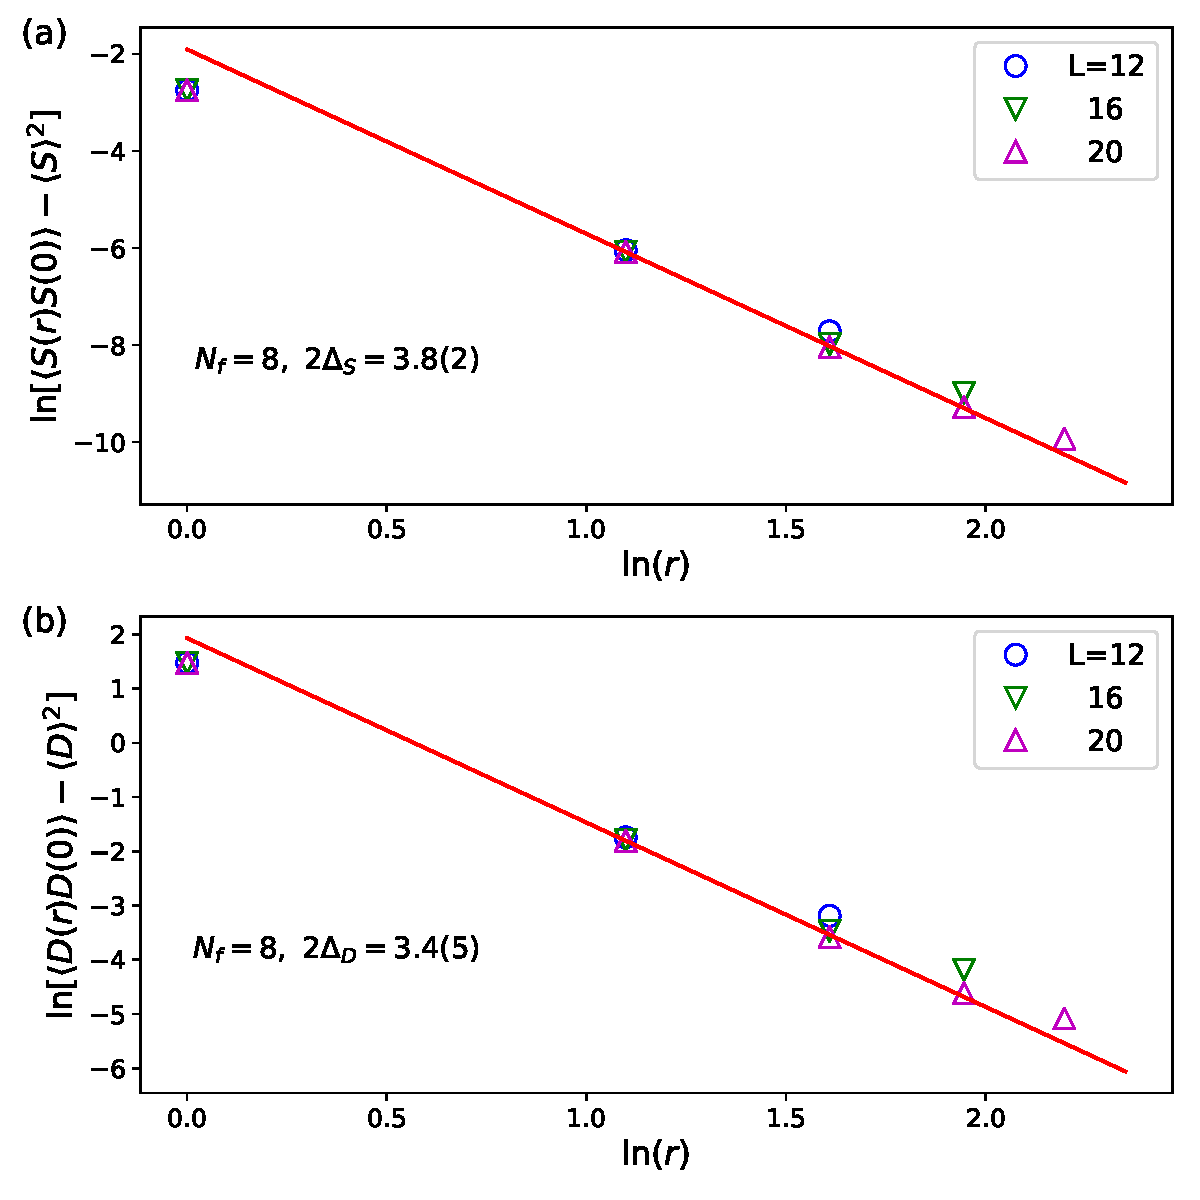
\includegraphics[width=\textwidth]{../u1sl/n8decay}
		\column{.5\textwidth}
		\begin{itemize}
			\item Spin and dimer OPs are fermion bilinears:
			\[\vec S = \psi^\dagger_{i\alpha}\vec\sigma_{\alpha\beta}\psi_{i\beta},\]
			\[D_{x,y} = \psi^\dagger_{i\alpha}\psi_{i+x,y,\beta}.\]
			\item Algebraic spin liquid: $\Delta_S = \Delta_D$.
		  \item (Free fermion has $\Delta_S=\Delta_D = 4$.)
		\end{itemize}
  \end{columns}
\end{frame}

\begin{frame}
  \frametitle{Summary}
  \begin{columns}
		\column{.7\textwidth}
    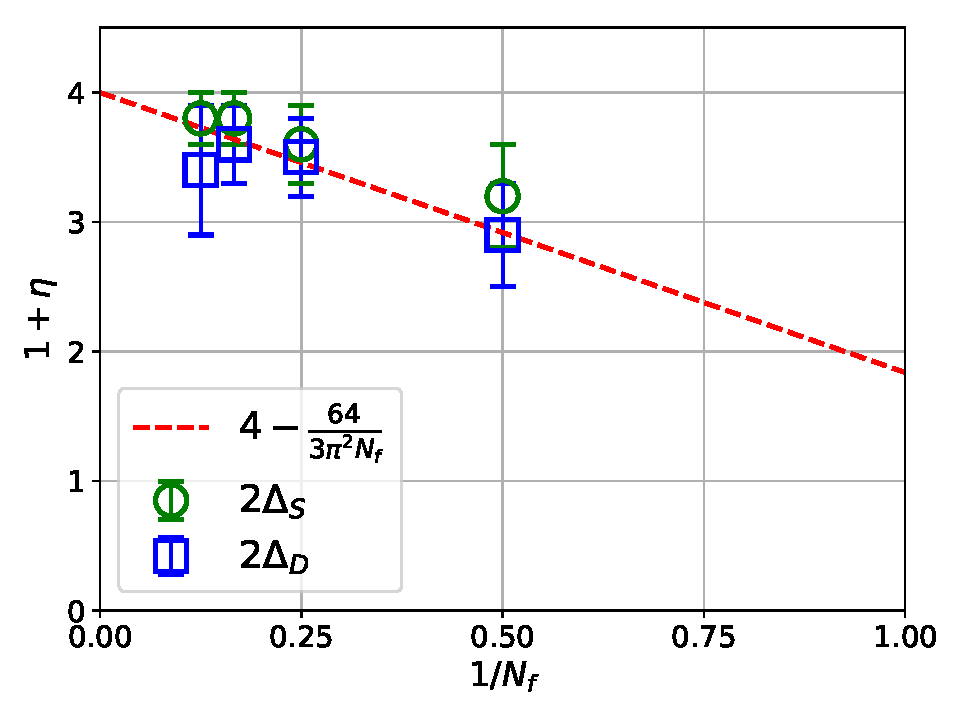
\includegraphics[width=\textwidth]{../u1sl/eta}
		\column{.3\textwidth}
		$\Delta_S=\Delta_D$ consistent with large-$N_f$-expansion results.
  \end{columns}
\end{frame}

\subsection{Conclusion}

\begin{frame}{Conclusion and outlooks}
  \begin{center}
    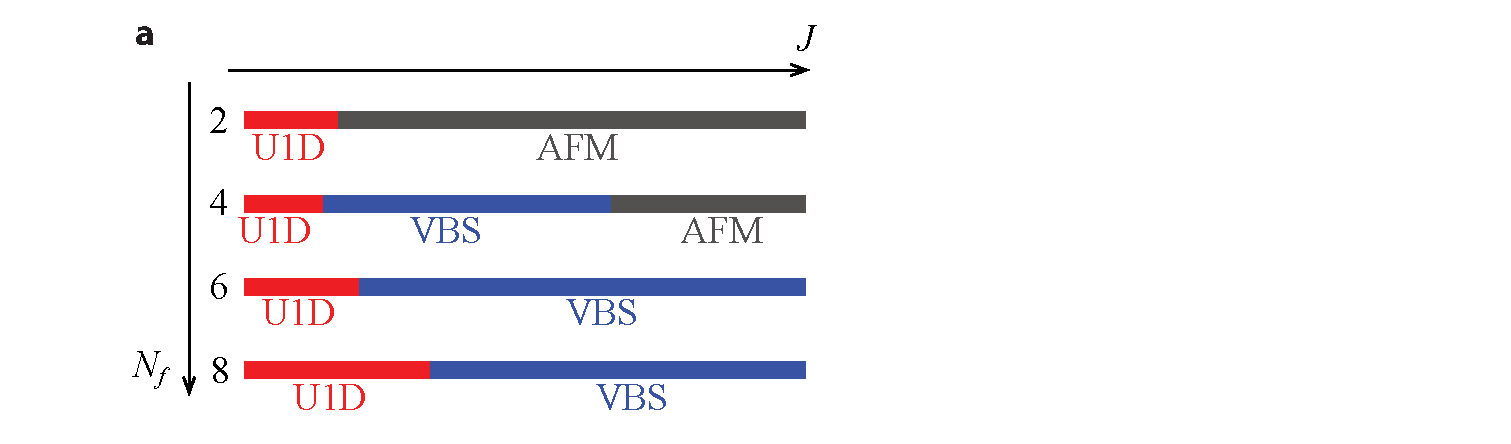
\includegraphics[width=5cm]{../u1sl/phase-diagram}

		{\small arXiv:1807.07574}
  \end{center}
  \begin{itemize}
    \item Deconfined U1D ASL phase observed for $N_f=2,4,6,8$.
    \item Confinement/deconfinement transition: continuous transition? universality class?
    \item Phase transition between VBS and AFM for $N_f=4$.
    \item Will U1D phase be stable in the IR limit? Larger sizes / directly measure monopole-operator scaling dimensions.
    \item Improving the algorithm: combining HMC / DQMC?
  \end{itemize}
\end{frame}

\section{Example: Orthogonal Metal}

\subsection{Introduction}


\begin{frame}
  \frametitle{Metal: Fermi surface}
\begin{itemize}
  \item Landau Fermi-Liquid Theory: a Fermi surface of quasiparticles.\\
  Noninteracting FS $\rightarrow$ Interacting FS.
  \item Volumn of the FS is conserved: Luttinger Thm.
\end{itemize}
\begin{center}
	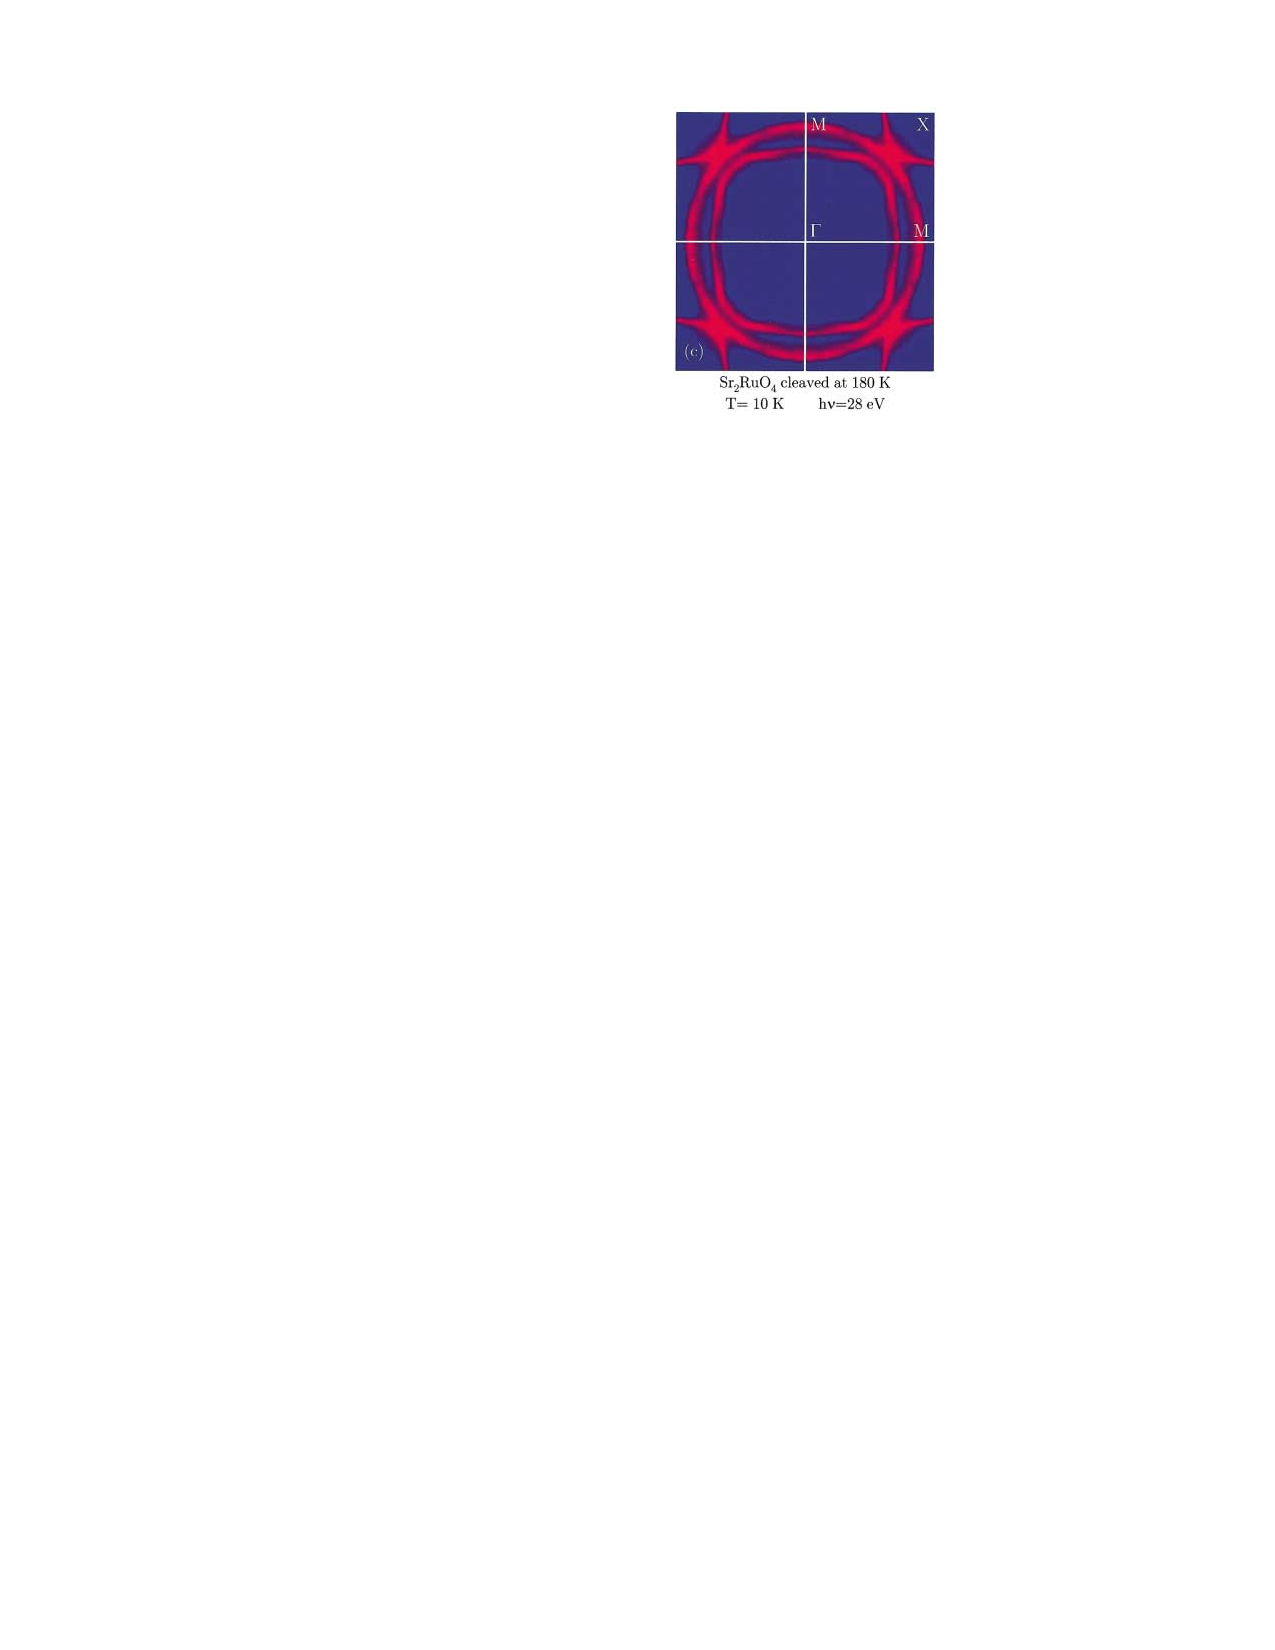
\includegraphics{../resources/SrRuO_FS}

	{\small A. Damascelli et al, PRL \textbf{85} 5194 (2000).}
\end{center}
\end{frame}

\begin{frame}
  \frametitle{Hiding an FS with Fractionalization}
  \begin{itemize}
    \item Spin-charge separation: $c_{i\alpha} = f_{i\alpha} h_i^\dagger$.
		\item $h$ forms a Mott insulator.
		\item No $c$-FS: no spectral weights.
		\item Generalized Luttinger Thm:
		$\nu_e = A_c + A_f$.
		\item Orthogonal metal: $\left<c^\dagger f\right>\rightarrow 0$.
  \end{itemize}
	\begin{center}
		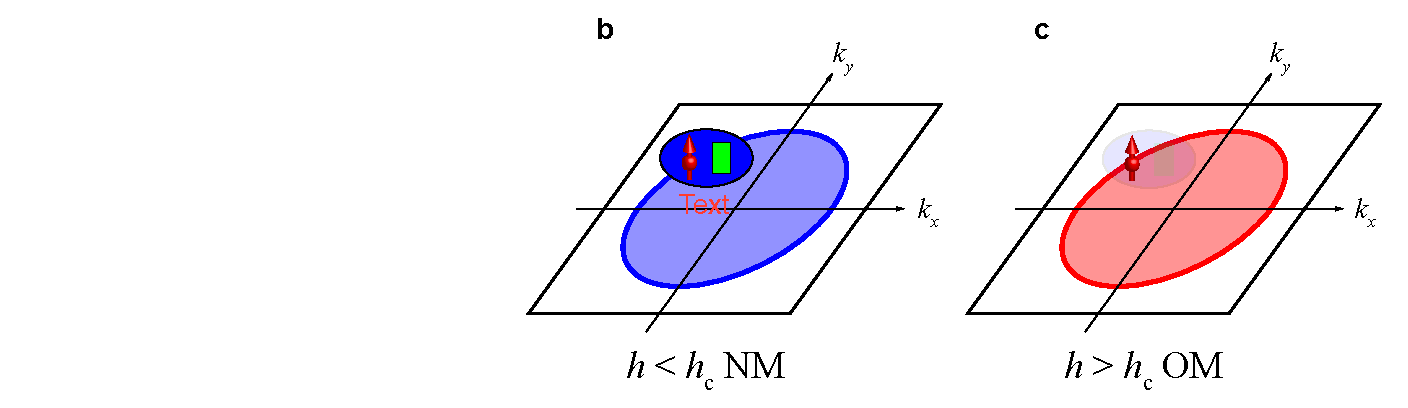
\includegraphics[width=.8\textwidth]{../orthogonal_metal/hide_fs}
	\end{center}
\end{frame}

\subsection{Model}

\begin{frame}
	\frametitle{The Model}
\begin{itemize}
\item Hamiltonian:
	\begin{align*}
	H_f &= -t\sum_{\langle i,j \rangle} (f^{\dagger}_{i,\alpha} \sigma^{z}_{b_{\langle i,j \rangle}}f_{j,\alpha} + h.c.) -\mu\sum_{i}f^{\dagger}_{i,\alpha}f_{i,\alpha}, \nonumber\\
	H_{z} &= -J \sum_{\langle i,j \rangle} S^{z}_{i} \sigma^{z}_{b_{\langle i,j \rangle}} S^{z}_{j} - h \sum_{i} S^{x}_{i}, \nonumber\\
	H_{g} &= -K \sum_{\square}\prod_{b\in\square} \sigma^{z}_{b} - g\sum_{b} \sigma^{x}_{b}.
\end{align*}
\item Physical fermion $c_{i\alpha} = f_{i\alpha}S_i^z$
\end{itemize}
\begin{center}
	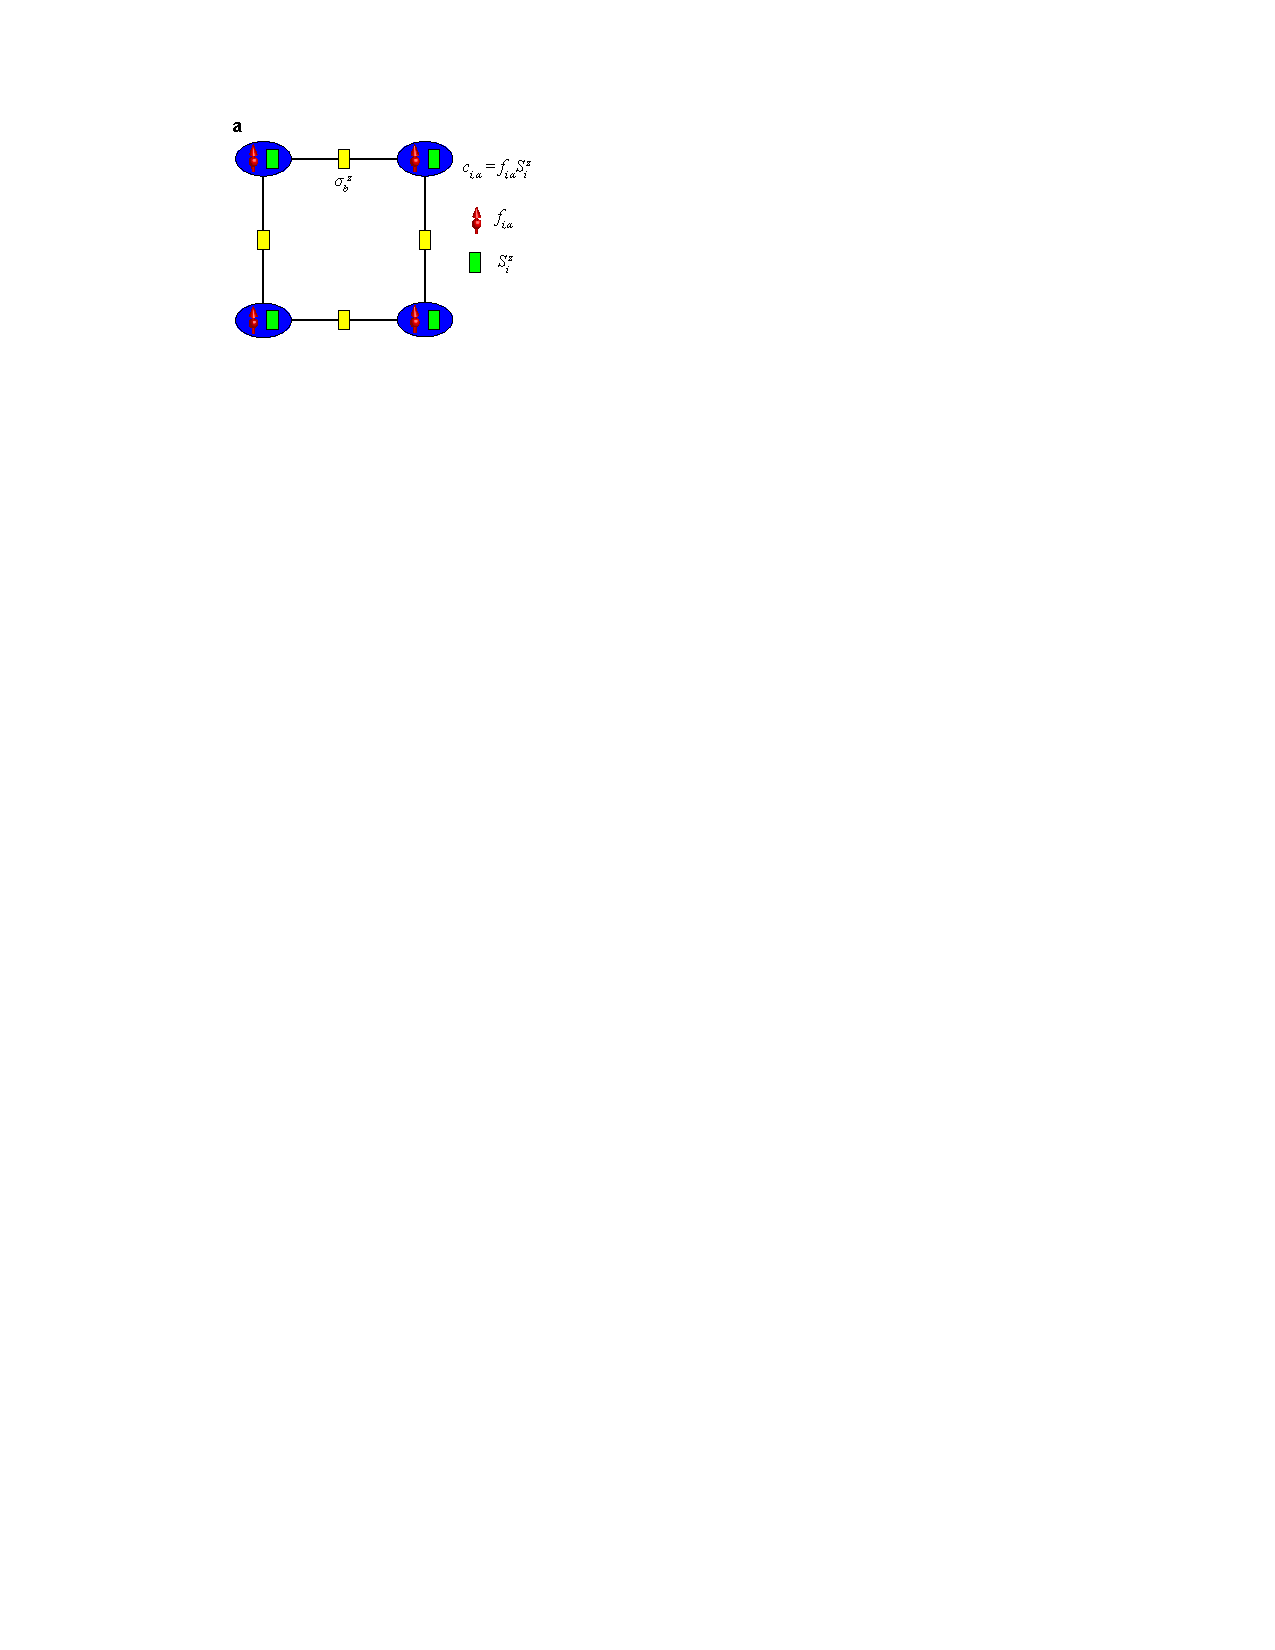
\includegraphics[width=4cm]{../orthogonal_metal/model_l}
\end{center}
\end{frame}

\begin{frame}
\frametitle{Symmetries -- I}
\begin{align*}
	H= &-t\sum_{\langle i,j \rangle} (f^{\dagger}_{i,\alpha} \sigma^{z}_{b_{\langle i,j \rangle}}f_{j,\alpha} + h.c.)
	-J \sum_{\langle i,j \rangle} S^{z}_{i} \sigma^{z}_{b_{\langle i,j \rangle}} S^{z}_{j} - h \sum_{i} S^{x}_{i}\\
&-K \sum_{\square}\prod_{b\in\square} \sigma^{z}_{b} - g\sum_{b} \sigma^{x}_{b}.
\end{align*}
\begin{enumerate}
\item $\mathbb Z_2$ gauge symmetry:
\[f_{i\alpha}\rightarrow\eta_if_{i\alpha},
\quad S_i^z\rightarrow\eta_iS_i^z,
\quad \sigma_{ij}\rightarrow
\eta_i\sigma_{ij}\eta_j.\]
\end{enumerate}
\begin{block}{Gauge constraint}
\begin{itemize}
\item Local projector $Q_i = (-)^{n_{i,f}}S^{x}_{i}\prod_{b\in +_i}\sigma^{x}_{b}$, w/ $n_{i,f}=\sum_{\alpha}f^{\dagger}_{i,\alpha}f_{i,\alpha}$.
\item $\hat Q_i=1$: Gauss Law.
\item $\hat Q_i\simeq1$ at low temperature: dynamically generated gauge-constraint.
\end{itemize}
\end{block}
\end{frame}

\begin{frame}
\frametitle{Symmetries -- II}
\begin{align*}
	H= &-t\sum_{\langle i,j \rangle} (f^{\dagger}_{i,\alpha} \sigma^{z}_{b_{\langle i,j \rangle}}f_{j,\alpha} + h.c.)
	-J \sum_{\langle i,j \rangle} S^{z}_{i} \sigma^{z}_{b_{\langle i,j \rangle}} S^{z}_{j} - h \sum_{i} S^{x}_{i}\\
&-K \sum_{\square}\prod_{b\in\square} \sigma^{z}_{b} - g\sum_{b} \sigma^{x}_{b}.
\end{align*}
\begin{enumerate}
	\addtocounter{enumi}{1}
\item $\mathbb Z_2$ \alert{global} symmetry:
$S_i^z\rightarrow -S_i^z$.
\item U(1) symmetry:
$f_{i\alpha}\rightarrow f_{i\alpha}e^{i\theta}$, $c_{i\alpha}\rightarrow c_{i\alpha}e^{i\theta}$.
$\Rightarrow$ Luttinger Theorem.
\end{enumerate}
\begin{block}{Ising symmetry is not really a global symmetry}
\begin{itemize}
\item Ising symmetry + fermion-parity symmetry $\in$ gauge symmetry:\\
$S_i^z\rightarrow-S_i^z,f_{i\alpha}\rightarrow-f_{i\alpha}$.
\item $\langle S_i^z\rangle\neq0$ is a \alert{Higgs} transition:
no\ bosonic local order parameter.
\end{itemize}
\end{block}
\end{frame}

\begin{frame}
\frametitle{Gauge symmetry and string operators}
\begin{itemize}
\item Gauge symmetry can never be broken.
\item Path integral / Monte Carlo sums over all gauge-equivalent configurations.
\item If $\hat O$ is not gauge invariant,
$\langle\hat O\rangle = 0$.
\item $\langle S_i^zS_j^z\rangle = 0$.
Need to use String operator $\langle S_i^z\sigma^z_{ii_1}\cdots\sigma^z_{i_nj}S_j^z\rangle$.
\item $\langle f_{i\alpha}f_{j\alpha}^\dagger\rangle=0$, $\langle c_{i\alpha}c_{j\alpha}^\dagger\rangle$ is Ok.
\end{itemize}

\begin{center}
	\begin{tikzpicture}
		\draw (0, 0)--(4, 0);
		\draw (0, 1)--(4, 1);
		\draw (0, 2)--(4, 2);
		\draw<1,3> (0, 3)--(4, 3);
		\draw (0, 4)--(4, 4);
		\draw (0, 0)--(0, 4);
		\draw (1, 0)--(1, 4);
		\draw (2, 0)--(2, 4);
		\draw<1,3> (3, 0)--(3, 4);
		\draw (4, 0)--(4, 4);
		\draw [thick,->,color=mbg] (0.9, 0.7)--(1.1, 1.3);
		\draw<1,3> [thick,->,color=mbg] (2.9, 2.7)--(3.1, 3.3);
		\draw<2> [thick,->,color=mbg] (3.1, 3.3)--(2.9, 2.7);
		\draw<2> [dashed] (2, 3)--(4, 3);
		\draw<2> (0, 3)--(2, 3);
		\draw<2> [dashed] (3, 2)--(3, 4);
		\draw<2> (3, 0)--(3, 2);
		\draw<3> [line width=2,blue] (1, 1)--(2, 1)--(2, 3)--(3, 3);
	\end{tikzpicture}
	\end{center}
\end{frame}

\subsection{Results}

\begin{frame}
\frametitle{Normal metal phase}
\begin{columns}
\column{.4\textwidth}
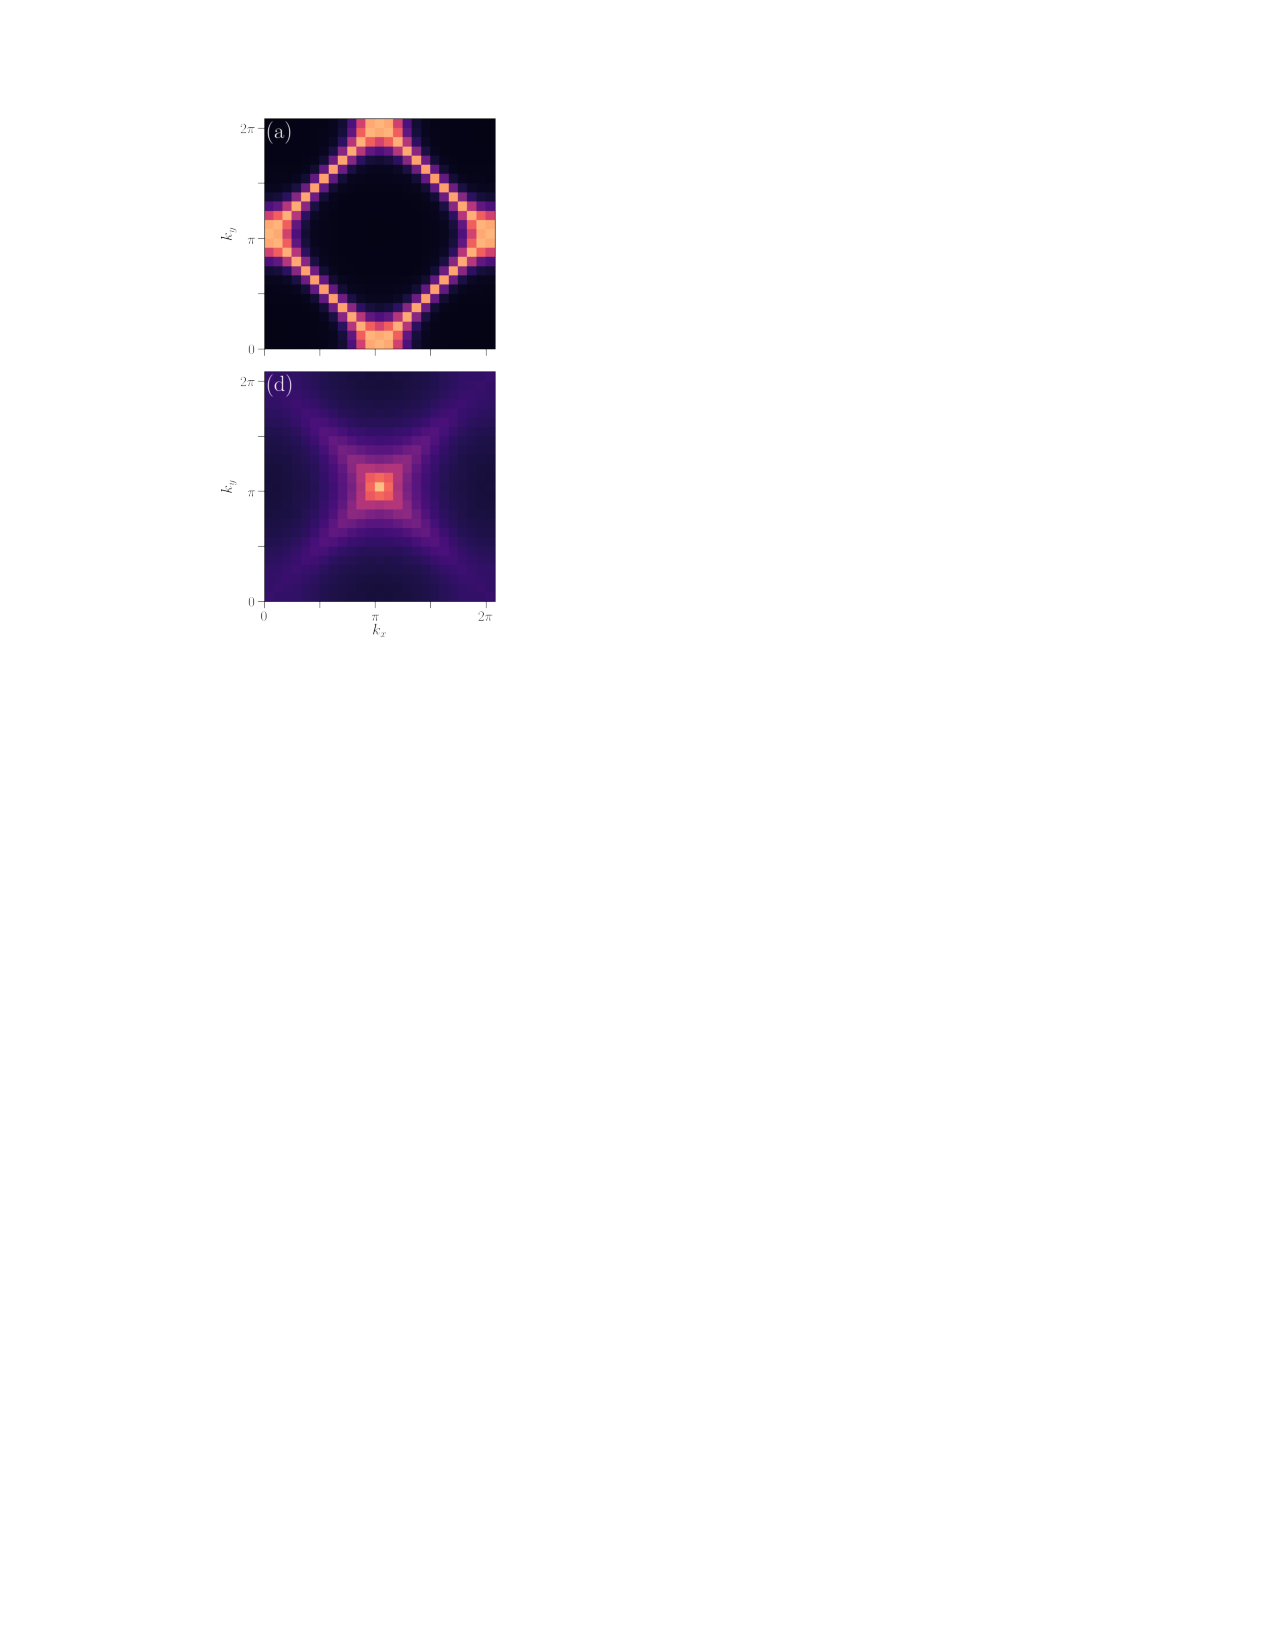
\includegraphics[width=\columnwidth]{../orthogonal_metal/nm}
\column{.6\textwidth}
\begin{itemize}
\item $h^z < h_c^z$: ``FM'' phase, ``$\langle S_i^z\rangle\neq0$''.
\item Higgs phase: $\mathbb Z_2$ gauge field is ``Higgs-ed''.
\item $c_{i\alpha} = S_i^zf_{i\alpha}\sim f_{i\alpha}$ forms a Fermi surface.
\item Susceptibility
$\chi_{ij}=\langle \vec s_i\cdot\vec s_j\rangle$,
$\vec s_i=c_{i\alpha}^\dagger\vec\sigma_{\alpha\beta}c_{i\beta}$ has a peak @ $(\pi,\pi)$.
\item A Landau Fermi liquid.
\end{itemize}
\end{columns}
\end{frame}

\begin{frame}
\frametitle{Orthogonal metal phase}
\begin{columns}
	\column{.4\textwidth}
	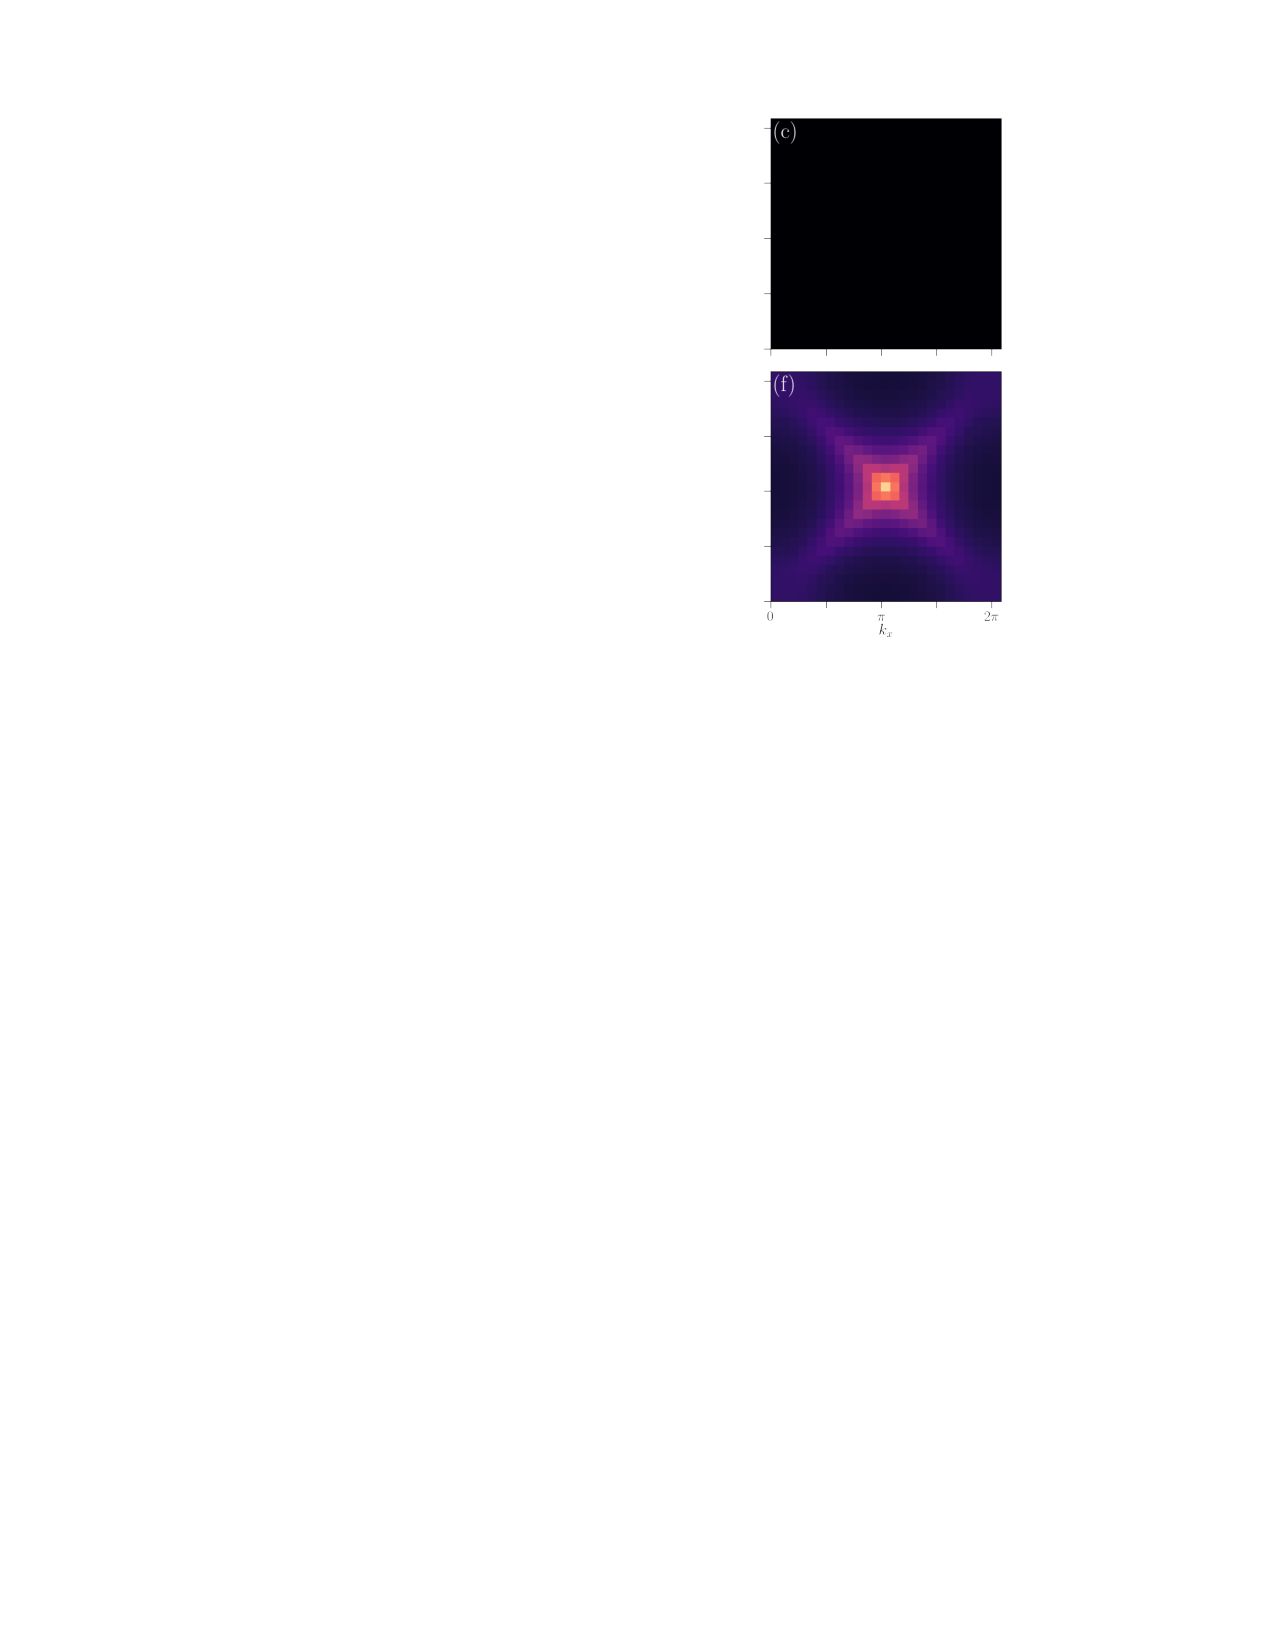
\includegraphics[width=.9\columnwidth]{../orthogonal_metal/om}
	\column{.6\textwidth}
	\begin{itemize}
	\item $h^z > h_c^z$: ``PM'' phase, ``$\langle S_i^z\rangle=0$''.
	\item $\mathbb Z_2$ gauge field is deconfined.
	\item Cannot find a $c$-fermion Fermi surface.
	\item Susceptibility still has a peak @ $(\pi,\pi)$: $\vec s_i= c_{i\alpha}^\dagger\vec\sigma_{\alpha\beta}c_{i\beta}
	= f_{i\alpha}^\dagger\vec\sigma_{\alpha\beta}f_{i\beta}$.
	\item A hidden $f$-fermion Fermi surface.
	\item A non-Fermi liquid: $\nu_e = A_f$ instead of $A_c$.
	\end{itemize}
\end{columns}
\end{frame}

\begin{frame}
\frametitle{Phase diagram}
\begin{itemize}
\item $c$-FS disappears.
\item Susceptibility peak remains $\Rightarrow$ a hidden $f$-FS.
\end{itemize}
\begin{center}
	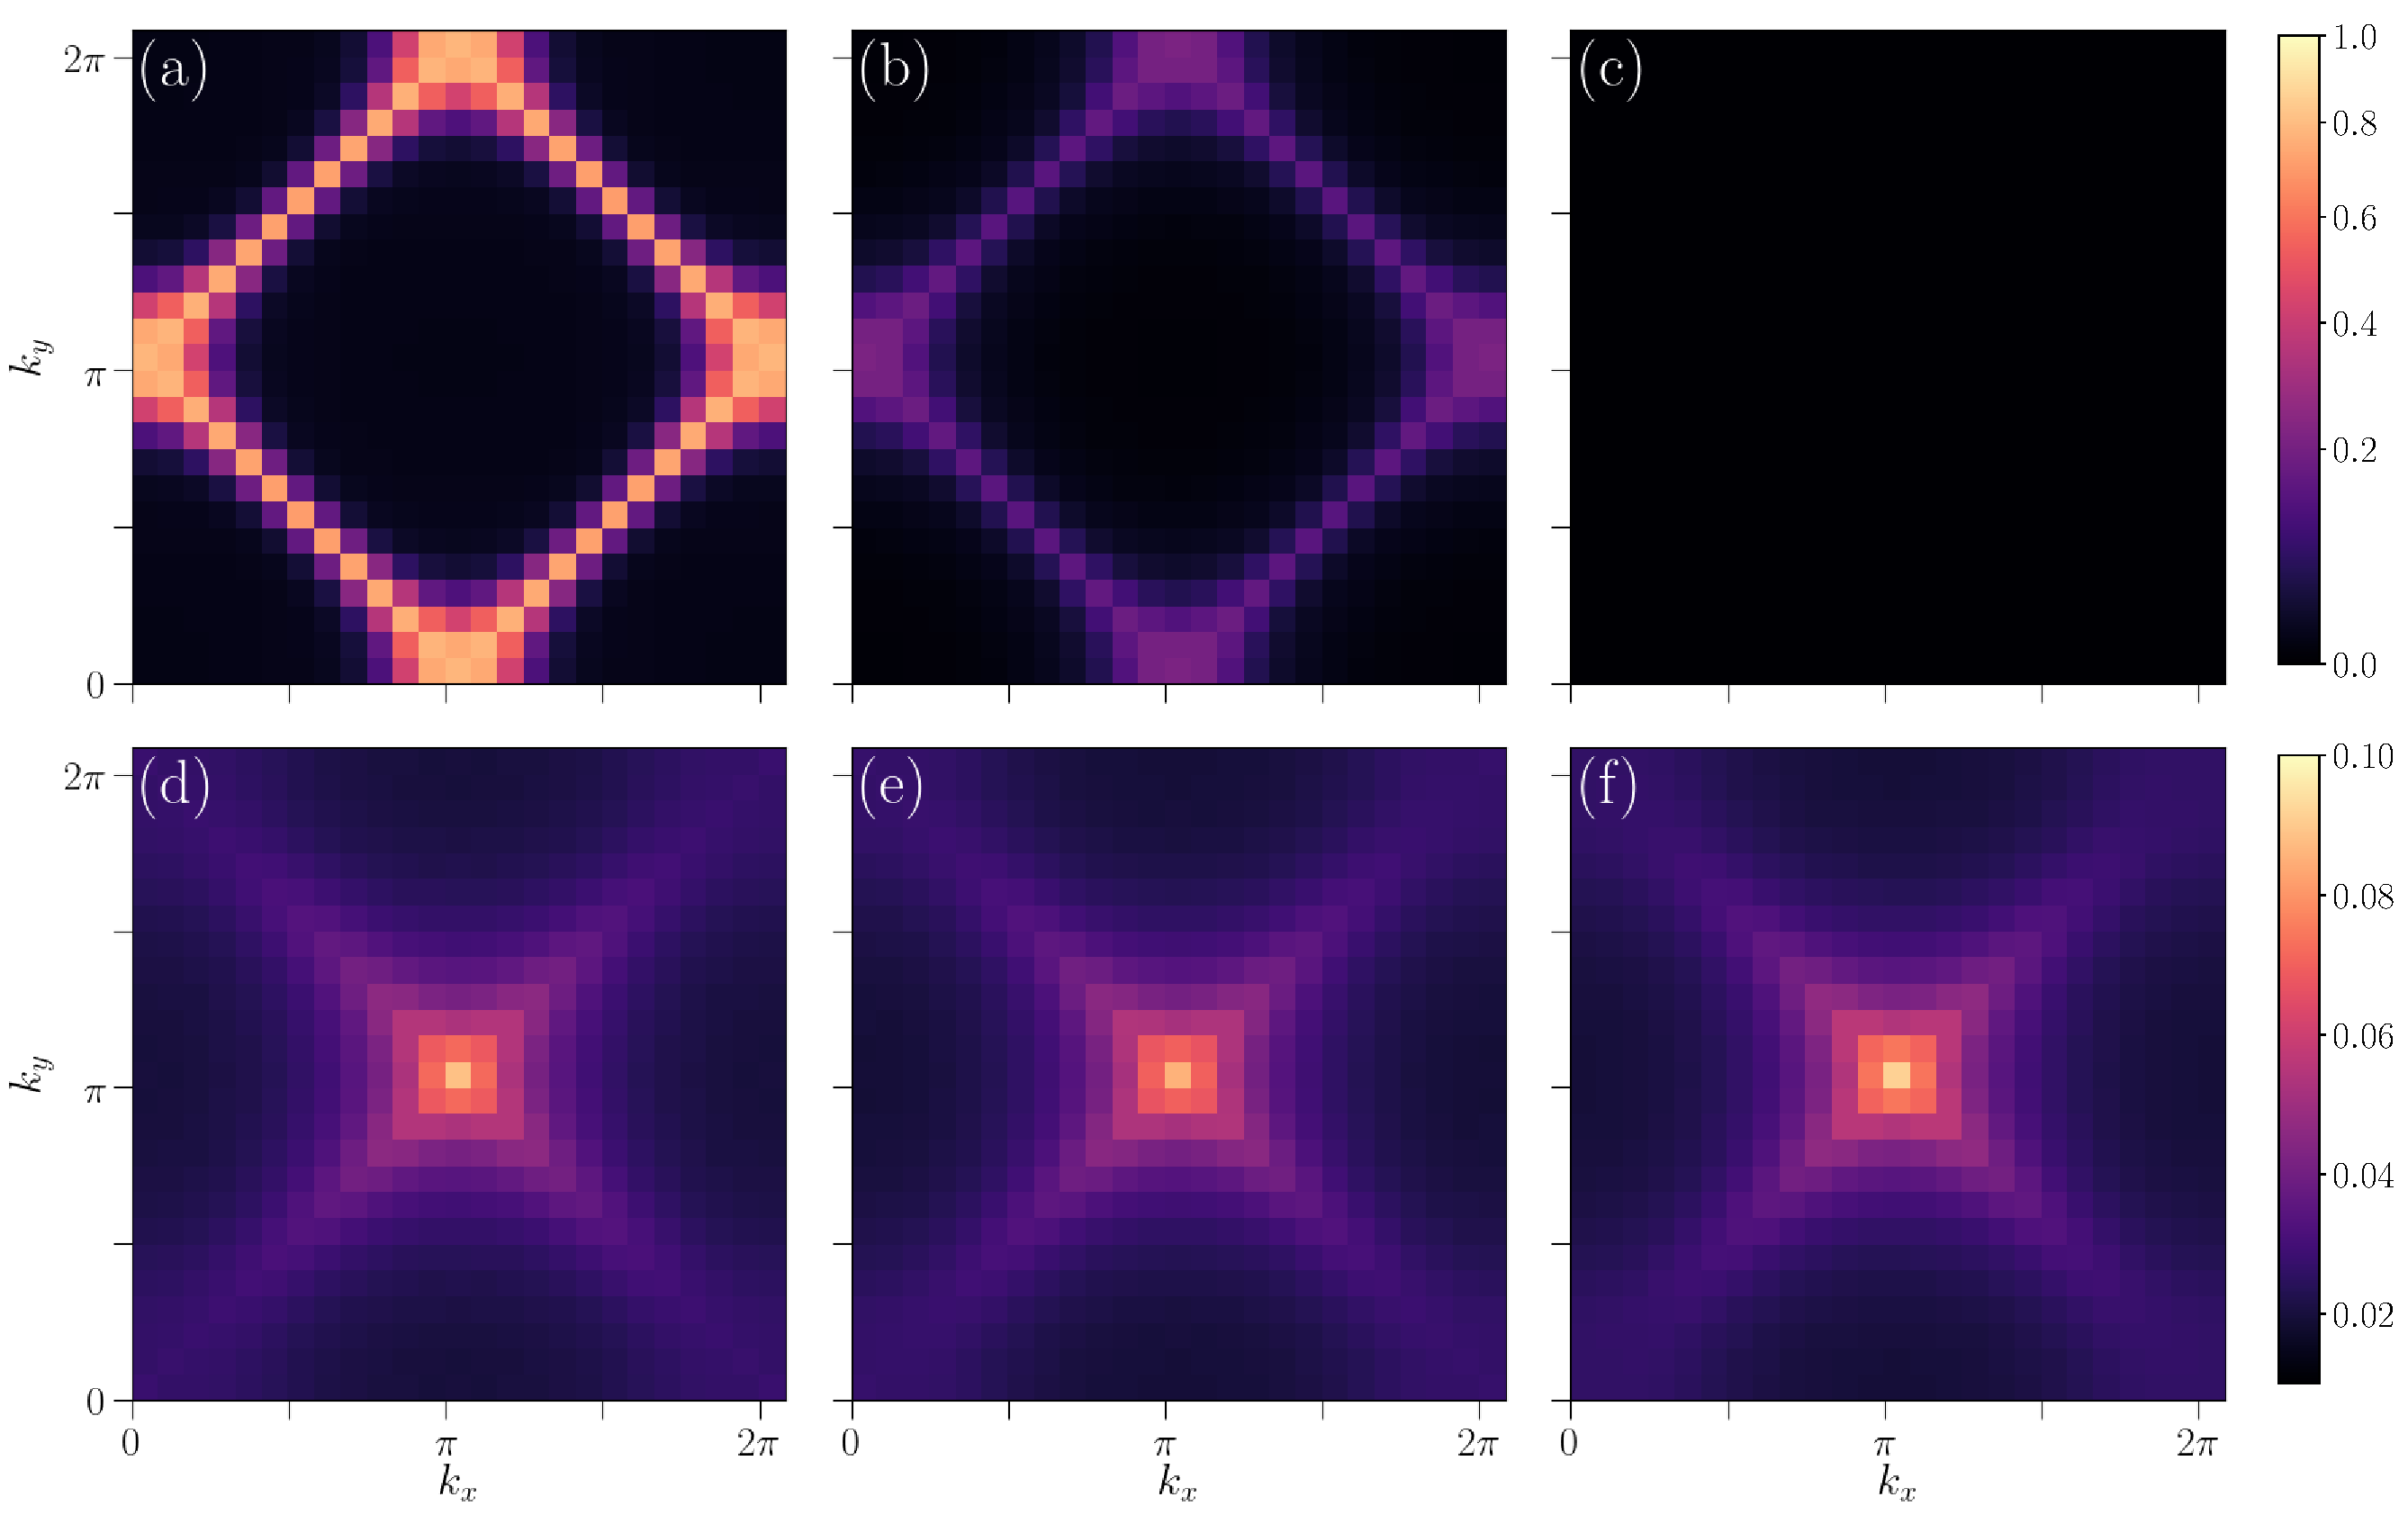
\includegraphics[width=\textwidth]{../orthogonal_metal/fig2}
\end{center}
\end{frame}

\begin{frame}
\frametitle{Phase diagram}
\begin{itemize}
\item $c$-FS disappears.
\item Susceptibility peak remains $\Rightarrow$ a hidden $f$-FS.
\end{itemize}
\begin{center}
	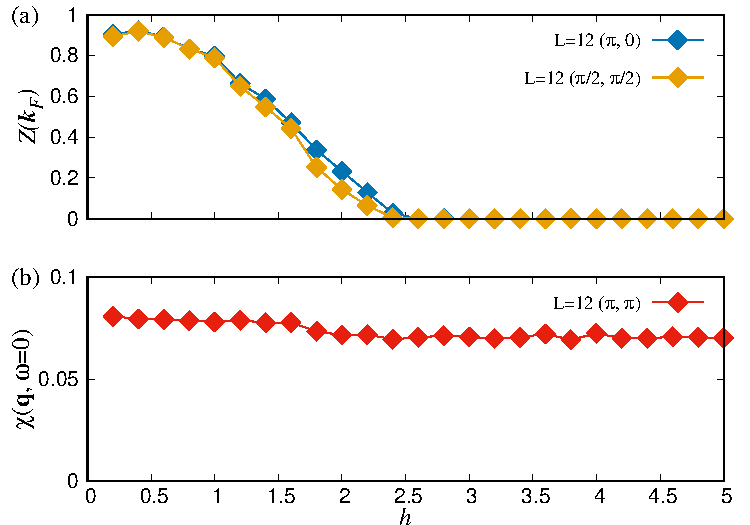
\includegraphics[width=.8\textwidth]{../orthogonal_metal/fig4}
\end{center}
\end{frame}

\begin{frame}
\frametitle{Away from half-filling}
\begin{center}
	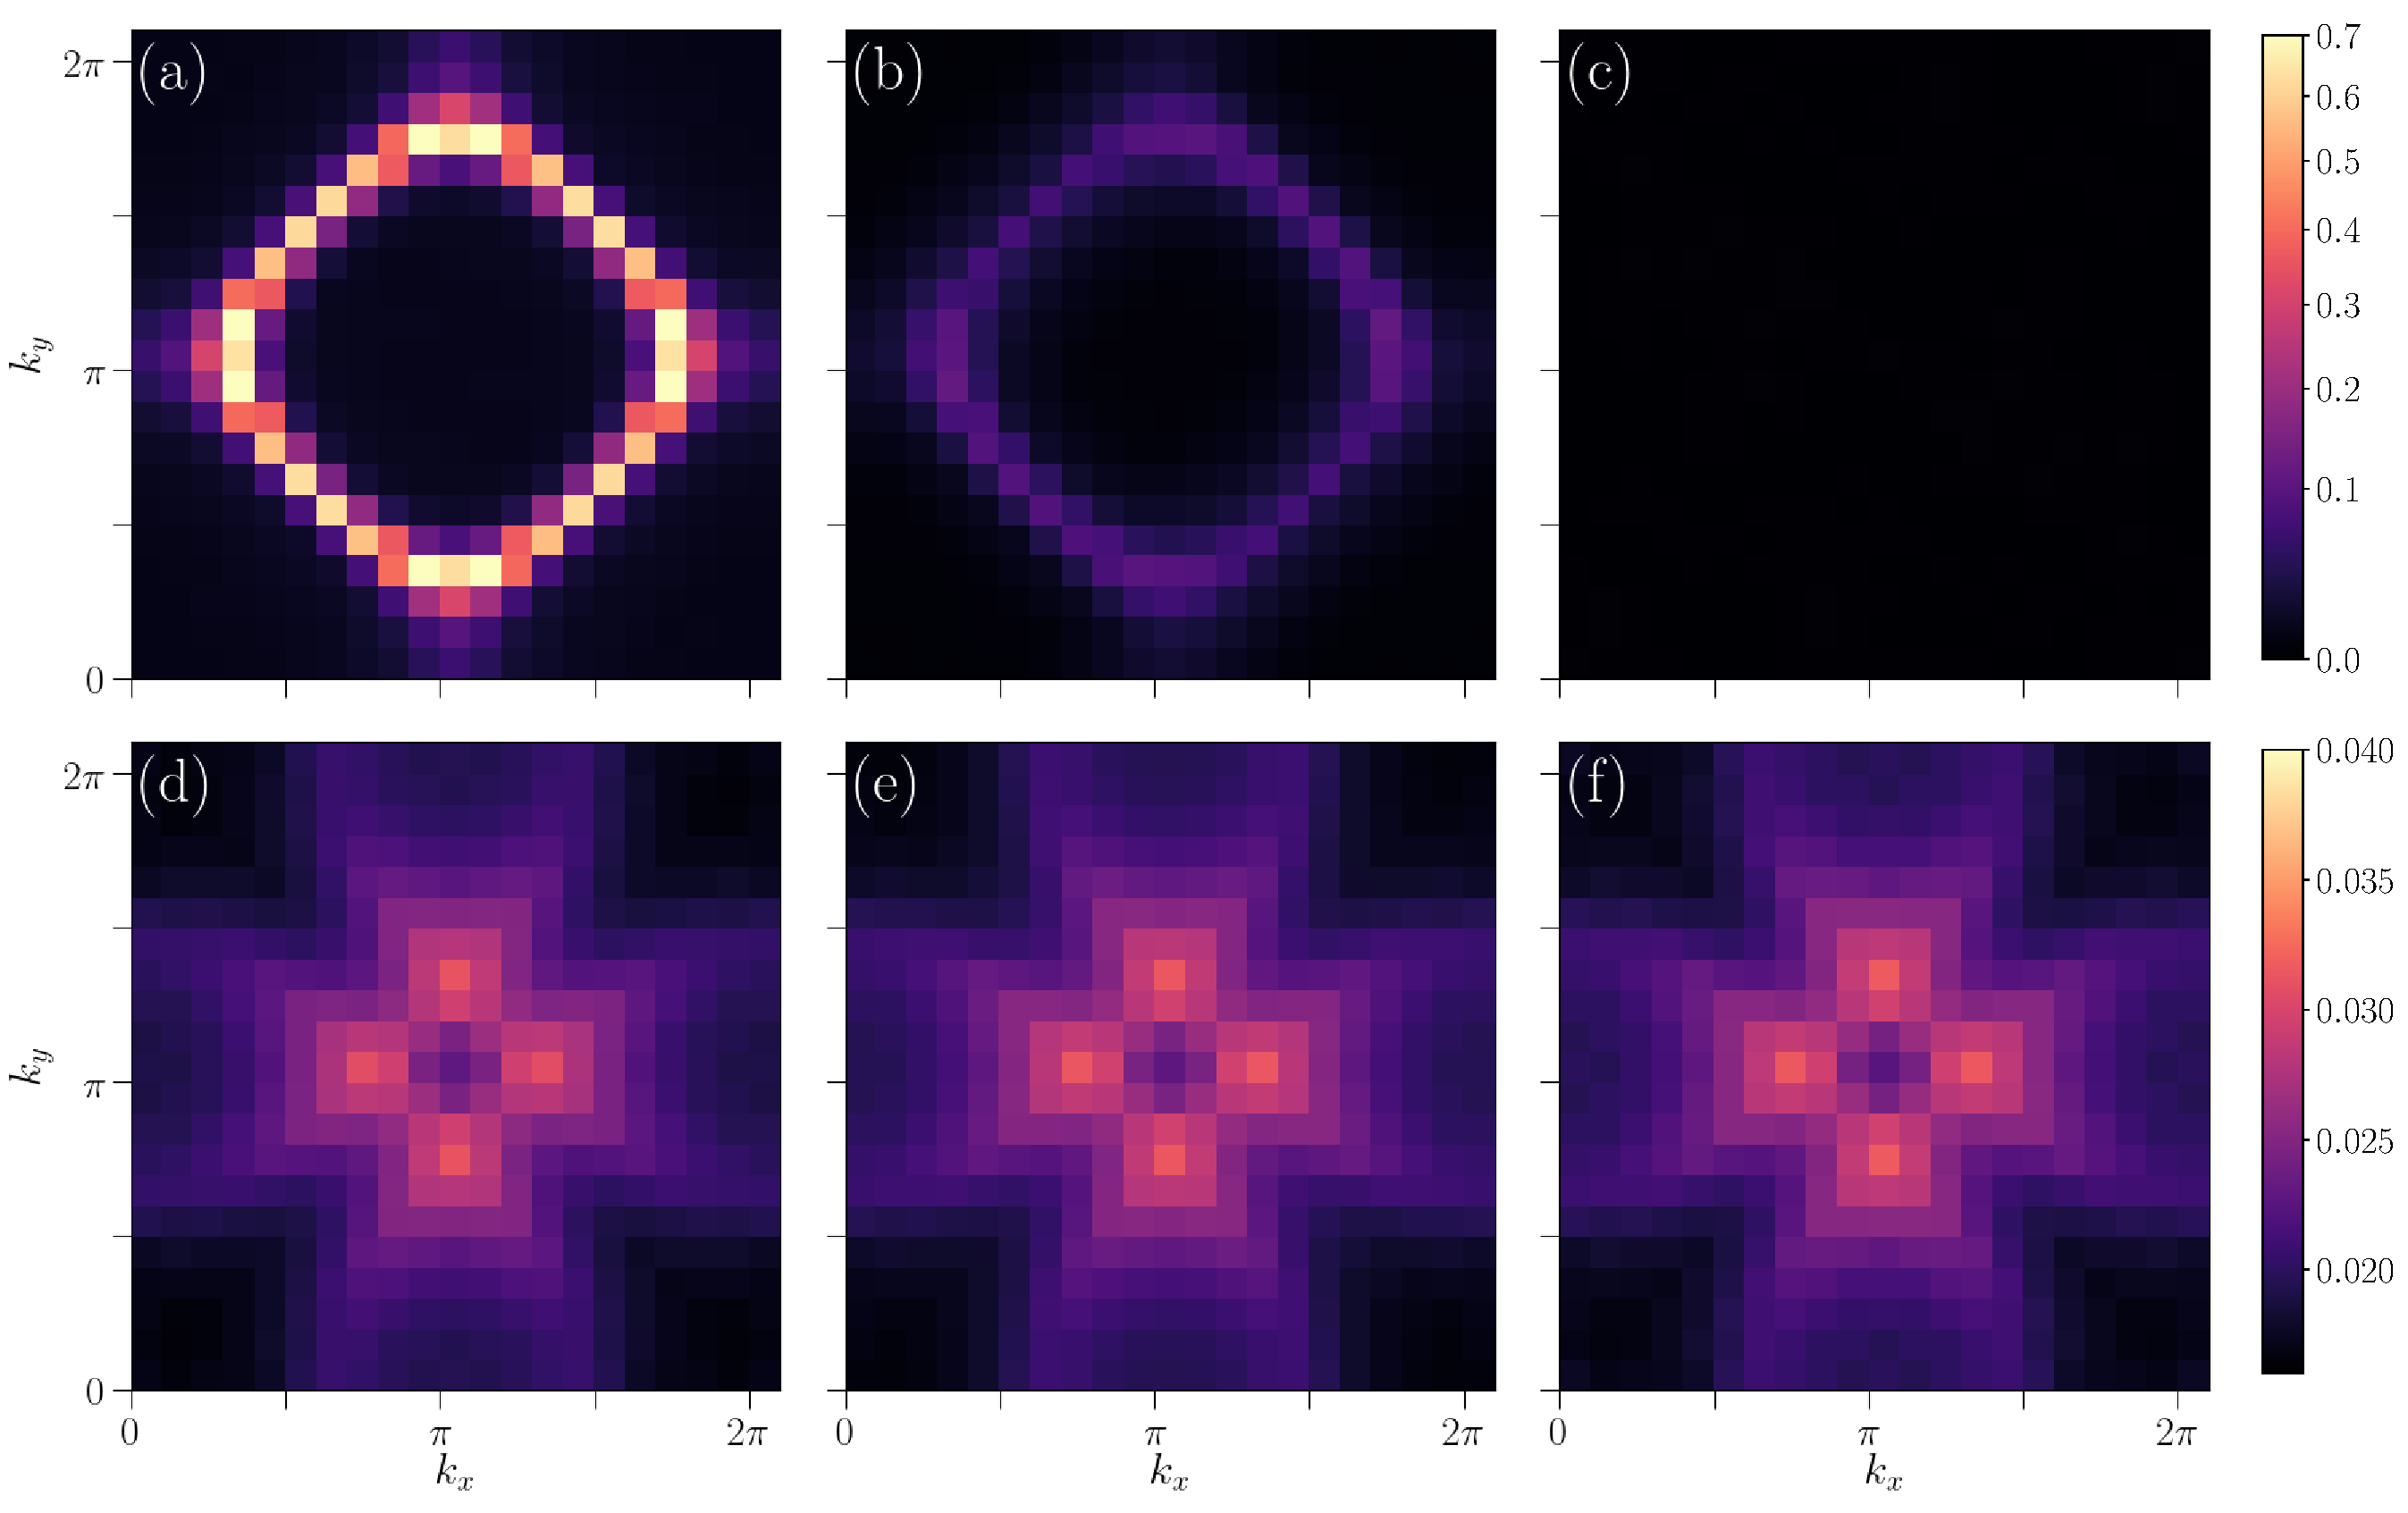
\includegraphics[width=\textwidth]{../orthogonal_metal/figS1}
\end{center}
\end{frame}

\begin{frame}
\frametitle{The Higgs transition}
\begin{center}
	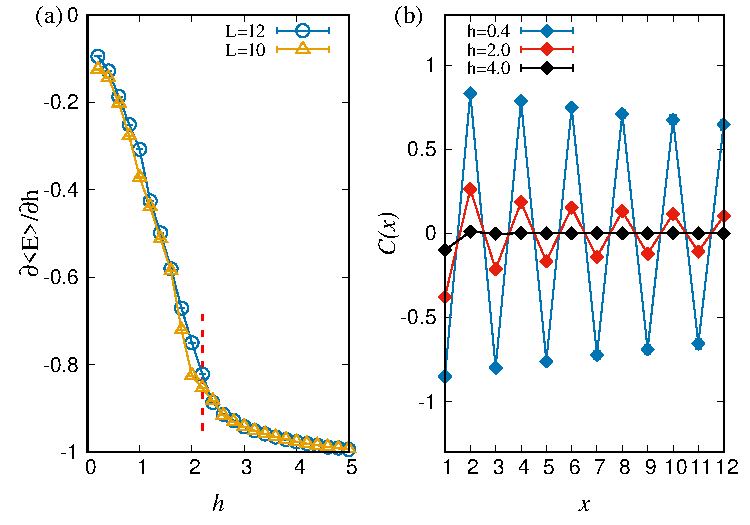
\includegraphics[height=5cm]{../orthogonal_metal/fig3}
\end{center}
\begin{itemize}
	\item Appears to be continuous.
	\item Hidden order: $\langle S_i^z\sigma^z\cdots\sigma^zS_j^z\rangle$.
	\item Not 3D Ising:
	$\mathcal L = (\partial_\mu\phi)^2-r\phi^2+u\phi^4+\phi^2\psi^\dagger\sigma^z\psi+\cdots$.
	\item Weak first-order? Sachdev and Morinari [PRB, 66, 235117 (2017)].
\end{itemize}
\end{frame}

\subsection{Conclusion}
\begin{frame}{Conclusion and Outlook}
\begin{center}
	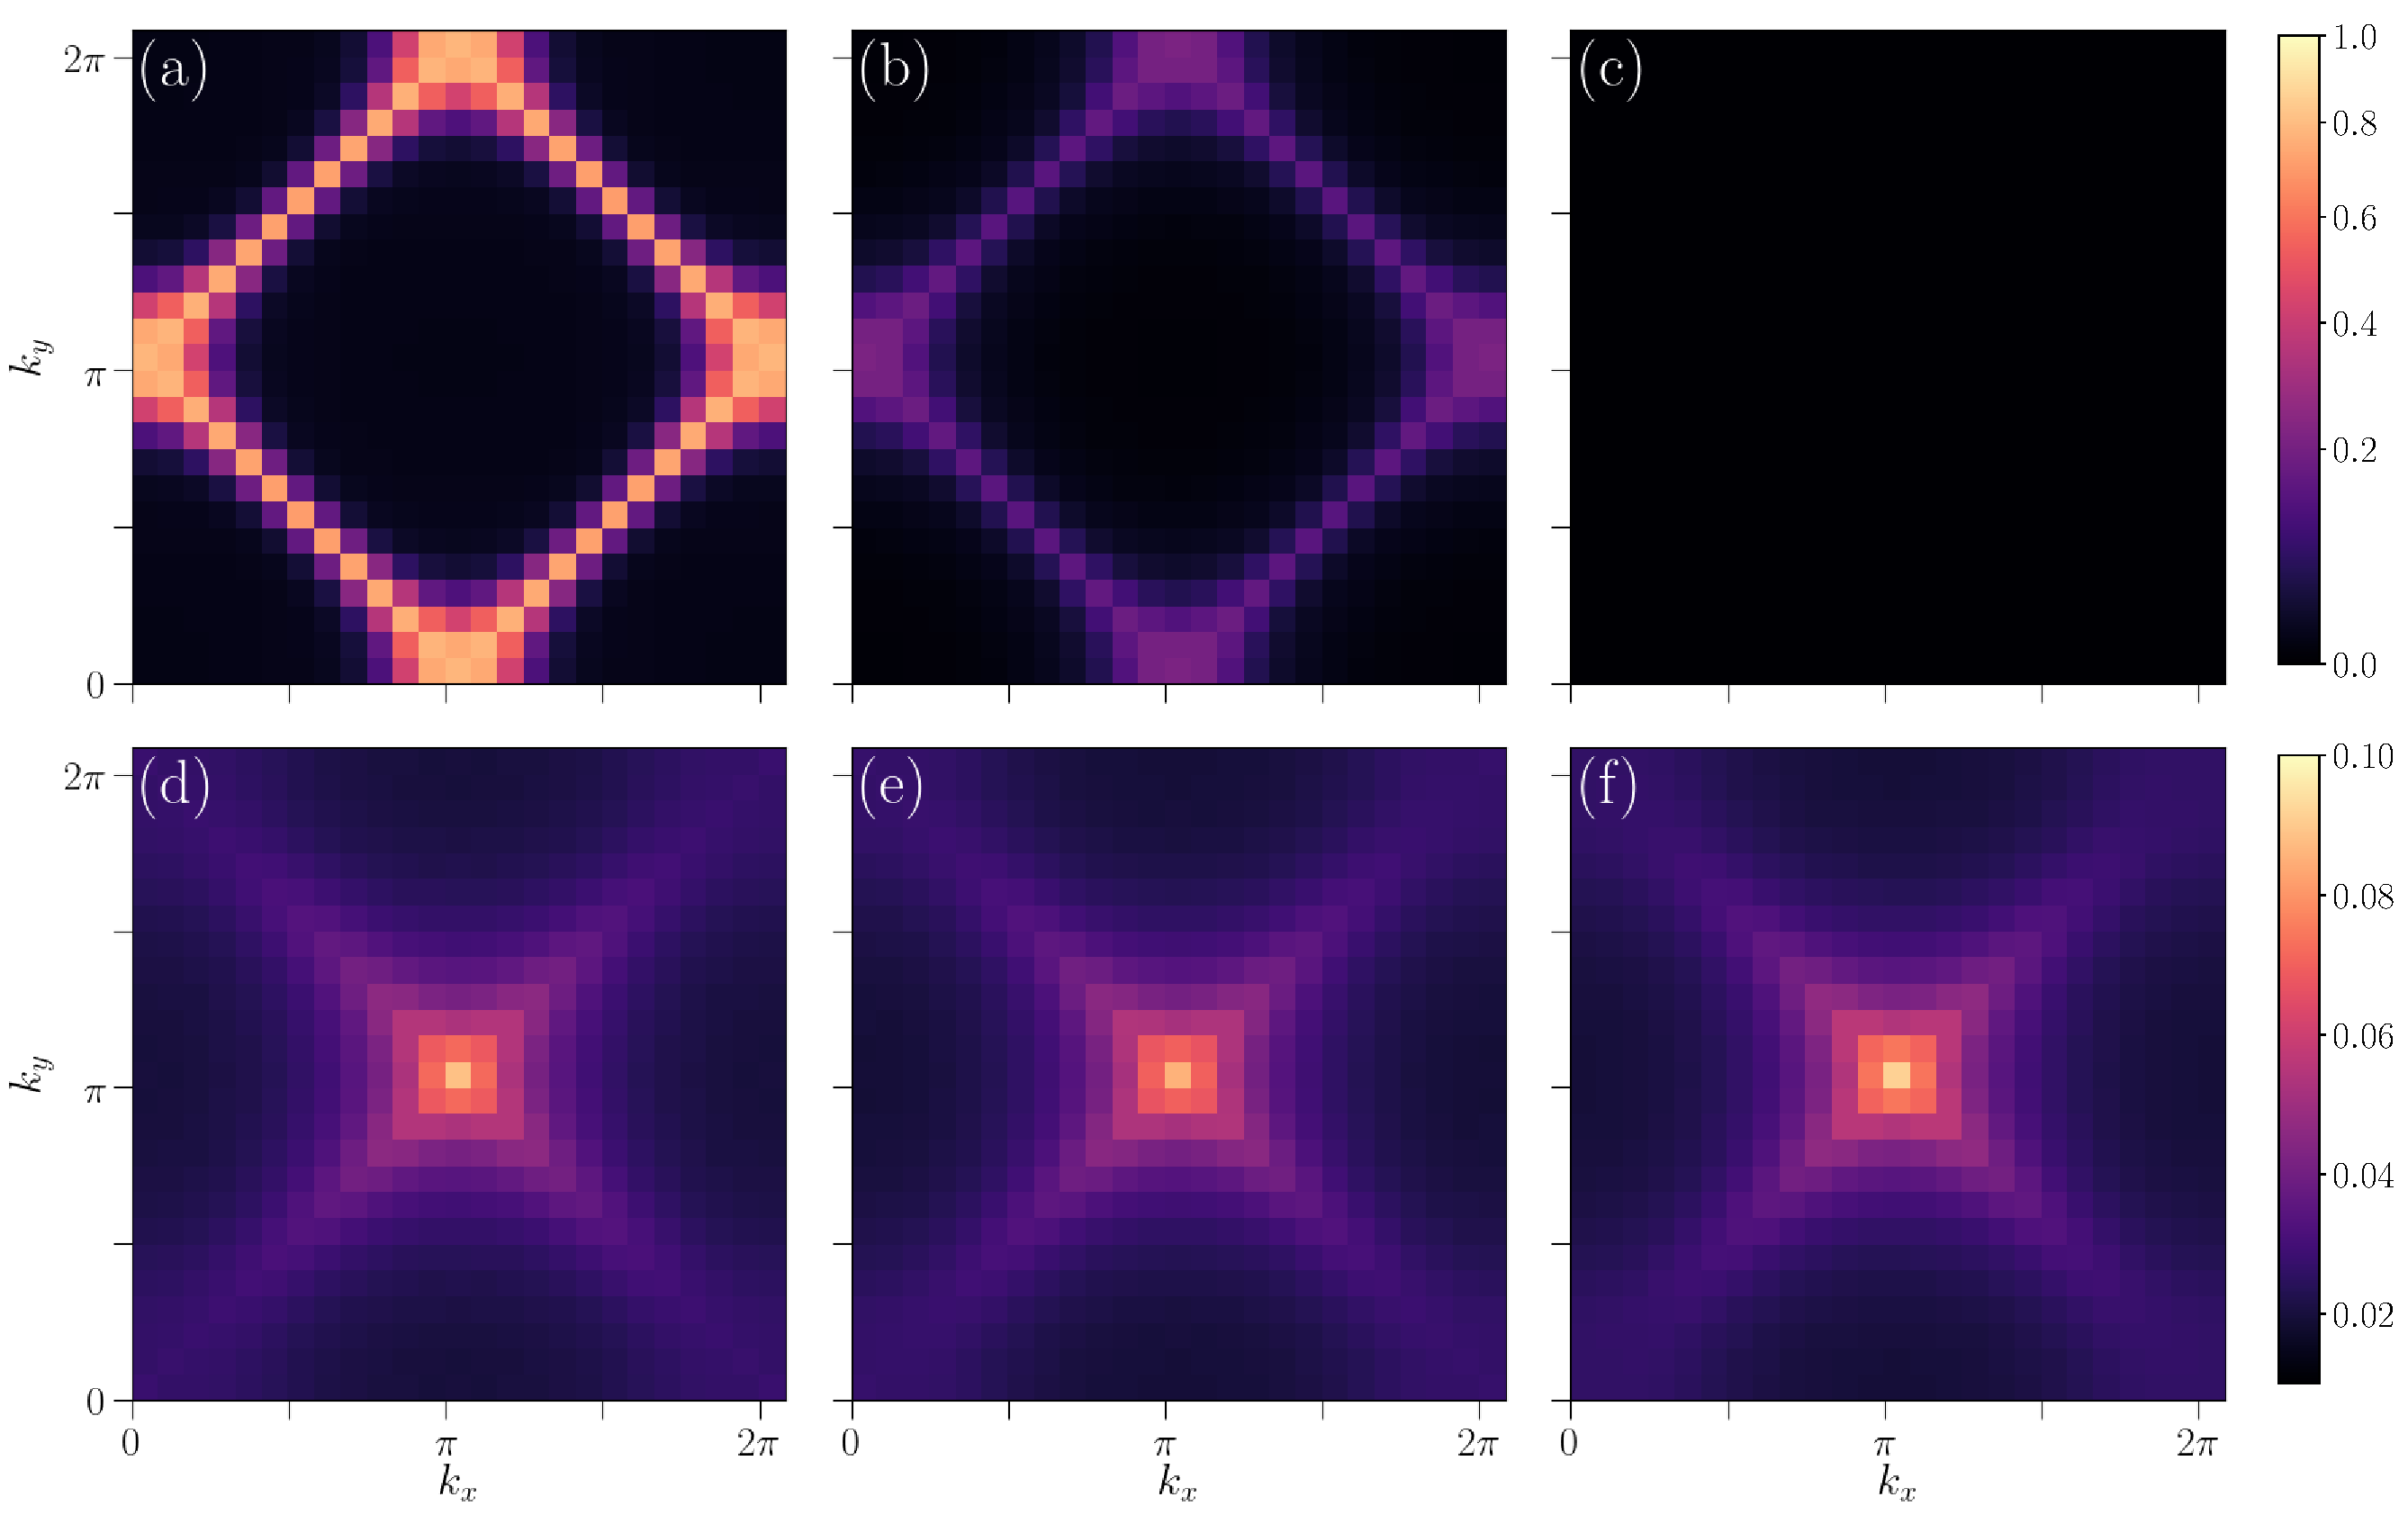
\includegraphics[width=.6\textwidth]{../orthogonal_metal/fig2}
\end{center}
\begin{itemize}
\item Metals' awkwark cousin is found.
\item Demonstrated an OM phase using MC simulation.
\item Higgs transition: appears to be continuous.
\item Spin liquid w/ spinon FS: U(1) spin liquid?
\item Nature of the phase transition?
\end{itemize}
\end{frame}

\end{document}
